%************************************************
\documentclass[ twoside,openright,titlepage,numbers=noenddot,headinclude,%1headlines,% letterpaper a4paper
                footinclude=true,cleardoublepage=empty,abstractoff, % <--- obsolete, remove (todo)
                BCOR=5mm,paper=a4,fontsize=11pt,%11pt,a4paper,%
                american,%
                ]{scrreprt}

%********************************************************************
% Note: Make all your adjustments in here
%*******************************************************
% ****************************************************************************************************
% classicthesis-config.tex 
% formerly known as loadpackages.sty, classicthesis-ldpkg.sty, and classicthesis-preamble.sty 
% Use it at the beginning of your ClassicThesis.tex, or as a LaTeX Preamble 
% in your ClassicThesis.{tex,lyx} with % ****************************************************************************************************
% classicthesis-config.tex 
% formerly known as loadpackages.sty, classicthesis-ldpkg.sty, and classicthesis-preamble.sty 
% Use it at the beginning of your ClassicThesis.tex, or as a LaTeX Preamble 
% in your ClassicThesis.{tex,lyx} with % ****************************************************************************************************
% classicthesis-config.tex 
% formerly known as loadpackages.sty, classicthesis-ldpkg.sty, and classicthesis-preamble.sty 
% Use it at the beginning of your ClassicThesis.tex, or as a LaTeX Preamble 
% in your ClassicThesis.{tex,lyx} with \input{classicthesis-config}
% ****************************************************************************************************  
% If you like the classicthesis, then I would appreciate a postcard. 
% My address can be found in the file ClassicThesis.pdf. A collection 
% of the postcards I received so far is available online at 
% http://postcards.miede.de
% ****************************************************************************************************


% ****************************************************************************************************
% 0. Set the encoding of your files. UTF-8 is the only sensible encoding nowadays. If you can't read
% äöüßáéçèê∂åëæƒÏ€ then change the encoding setting in your editor, not the line below. If your editor
% does not support utf8 use another editor!
% ****************************************************************************************************
\PassOptionsToPackage{utf8}{inputenc}
	\usepackage{inputenc}

% ****************************************************************************************************
% 1. Configure classicthesis for your needs here, e.g., remove "drafting" below 
% in order to deactivate the time-stamp on the pages
% ****************************************************************************************************
\PassOptionsToPackage{eulerchapternumbers,listings,drafting,%
					 pdfspacing,%floatperchapter,%linedheaders,%
					 subfig,beramono,eulermath,parts}{classicthesis}                                        
% ********************************************************************
% Available options for classicthesis.sty 
% (see ClassicThesis.pdf for more information):
% drafting
% parts nochapters linedheaders
% eulerchapternumbers beramono eulermath pdfspacing minionprospacing
% tocaligned dottedtoc manychapters
% listings floatperchapter subfig
% ********************************************************************


% ****************************************************************************************************
% 2. Personal data and user ad-hoc commands
% ****************************************************************************************************
\newcommand{\myTitle}{Planets orbiting evolving binary stars\xspace}
\newcommand{\mySubtitle}{Subtitle\xspace}
%\newcommand{\myDegree}{Doktor-Ingenieur (Dr.-Ing.)\xspace}
\newcommand{\myName}{Fran Bartolić\xspace}
\newcommand{\myProf}{Put name here\xspace}
\newcommand{\myOtherProf}{Put name here\xspace}
\newcommand{\mySupervisor}{Put name here\xspace}
\newcommand{\myFaculty}{Put data here\xspace}
\newcommand{\myDepartment}{Put data here\xspace}
\newcommand{\myUni}{Department of Physics, University of Rijeka\xspace}
\newcommand{\myLocation}{Rijeka, Croatia\xspace}
\newcommand{\myTime}{July 2017\xspace}
%\newcommand{\myVersion}{version 4.2\xspace}

% ********************************************************************
% Setup, finetuning, and useful commands
% ********************************************************************
\newcounter{dummy} % necessary for correct hyperlinks (to index, bib, etc.)
\newlength{\abcd} % for ab..z string length calculation
\providecommand{\mLyX}{L\kern-.1667em\lower.25em\hbox{Y}\kern-.125emX\@}
\newcommand{\ie}{i.\,e.}
\newcommand{\Ie}{I.\,e.}
\newcommand{\eg}{e.\,g.}
\newcommand{\Eg}{E.\,g.} 
% ****************************************************************************************************


% ****************************************************************************************************
% 3. Loading some handy packages
% ****************************************************************************************************
% ******************************************************************** 
% Packages with options that might require adjustments
% ******************************************************************** 
%\PassOptionsToPackage{ngerman,american}{babel}   % change this to your language(s)
% Spanish languages need extra options in order to work with this template
%\PassOptionsToPackage{spanish,es-lcroman}{babel}
	\usepackage{babel}                  

\usepackage{csquotes}
\PassOptionsToPackage{%
    %backend=biber, %instead of bibtex
	backend=bibtex8,bibencoding=ascii,%
	language=auto,%
	style=numeric-comp,%
    %style=authoryear-comp, % Author 1999, 2010
    %bibstyle=authoryear,dashed=false, % dashed: substitute rep. author with ---
    sorting=nyt, % name, year, title
    maxbibnames=10, % default: 3, et al.
    %backref=true,%
    natbib=true % natbib compatibility mode (\citep and \citet still work)
}{biblatex}
    \usepackage{biblatex}

\PassOptionsToPackage{fleqn}{amsmath}       % math environments and more by the AMS 
    \usepackage{amsmath}

\usepackage{siunitx} % for physical units
\newcommand{\vect}[1]{\boldsymbol{\mathbf{#1}}} % shorthand for bold vectors
% ******************************************************************** 
% General useful packages
% ******************************************************************** 
\PassOptionsToPackage{T1}{fontenc} % T2A for cyrillics
    \usepackage{fontenc}     
\usepackage{textcomp} % fix warning with missing font shapes
\usepackage{scrhack} % fix warnings when using KOMA with listings package          
\usepackage{xspace} % to get the spacing after macros right  
\usepackage{mparhack} % get marginpar right
%\usepackage[latest]{latexrelease} % will be used once available in more distributions (ISSUE #107)
\PassOptionsToPackage{printonlyused,smaller}{acronym} 
    \usepackage{acronym} % nice macros for handling all acronyms in the thesis
    %\renewcommand{\bflabel}[1]{{#1}\hfill} % fix the list of acronyms --> no longer working
    %\renewcommand*{\acsfont}[1]{\textsc{#1}} 
    \renewcommand*{\aclabelfont}[1]{\acsfont{#1}}
% ****************************************************************************************************


% ****************************************************************************************************
% 4. Setup floats: tables, (sub)figures, and captions
% ****************************************************************************************************
%\usepackage{tabularx} % better tables
%    \setlength{\extrarowheight}{3pt} % increase table row height
\usepackage{booktabs} % better tables
\renewcommand{\arraystretch}{1.3} (or 1.3)
\newcommand{\tableheadline}[1]{\multicolumn{1}{c}{\spacedlowsmallcaps{#1}}}
\newcommand{\myfloatalign}{\centering} % to be used with each float for alignment
\usepackage{caption}
% Thanks to cgnieder and Claus Lahiri
% http://tex.stackexchange.com/questions/69349/spacedlowsmallcaps-in-caption-label
% [REMOVED DUE TO OTHER PROBLEMS, SEE ISSUE #82]    
%\DeclareCaptionLabelFormat{smallcaps}{\bothIfFirst{#1}{~}\MakeTextLowercase{\textsc{#2}}}
%\captionsetup{font=small,labelformat=smallcaps} % format=hang,
\captionsetup{font=small} % format=hang,
\usepackage{subfig}  
% ****************************************************************************************************


% ****************************************************************************************************
% 5. Setup code listings
% ****************************************************************************************************
\usepackage{listings} 
%\lstset{emph={trueIndex,root},emphstyle=\color{BlueViolet}}%\underbar} % for special keywords
\lstset{language=[LaTeX]Tex,%C++,
    morekeywords={PassOptionsToPackage,selectlanguage},
    keywordstyle=\color{RoyalBlue},%\bfseries,
    basicstyle=\small\ttfamily,
    %identifierstyle=\color{NavyBlue},
    commentstyle=\color{Green}\ttfamily,
    stringstyle=\rmfamily,
    numbers=none,%left,%
    numberstyle=\scriptsize,%\tiny
    stepnumber=5,
    numbersep=8pt,
    showstringspaces=false,
    breaklines=true,
    %frameround=ftff,
    %frame=single,
    belowcaptionskip=.75\baselineskip
    %frame=L
} 
% ****************************************************************************************************             


% ****************************************************************************************************
% 6. PDFLaTeX, hyperreferences and citation backreferences
% ****************************************************************************************************
% ********************************************************************
% Using PDFLaTeX
% ********************************************************************
\PassOptionsToPackage{pdftex,hyperfootnotes=false,pdfpagelabels}{hyperref}
    \usepackage{hyperref}  % backref linktocpage pagebackref
\pdfcompresslevel=9
\pdfadjustspacing=1 
\PassOptionsToPackage{pdftex}{graphicx}
    \usepackage{graphicx} 
 

% ********************************************************************
% Hyperreferences
% ********************************************************************
\hypersetup{%
    %draft, % = no hyperlinking at all (useful in b/w printouts)
    colorlinks=true, linktocpage=true, pdfstartpage=3, pdfstartview=FitV,%
    % uncomment the following line if you want to have black links (e.g., for printing)
    %colorlinks=false, linktocpage=false, pdfstartpage=3, pdfstartview=FitV, pdfborder={0 0 0},%
    breaklinks=true, pdfpagemode=UseNone, pageanchor=true, pdfpagemode=UseOutlines,%
    plainpages=false, bookmarksnumbered, bookmarksopen=true, bookmarksopenlevel=1,%
    hypertexnames=true, pdfhighlight=/O,%nesting=true,%frenchlinks,%
    urlcolor=webbrown, linkcolor=RoyalBlue, citecolor=webgreen, %pagecolor=RoyalBlue,%
    %urlcolor=Black, linkcolor=Black, citecolor=Black, %pagecolor=Black,%
    pdftitle={\myTitle},%
    pdfauthor={\textcopyright\ \myName, \myUni, \myFaculty},%
    pdfsubject={},%
    pdfkeywords={},%
    pdfcreator={pdfLaTeX},%
    pdfproducer={LaTeX with hyperref and classicthesis}%
}   
\usepackage{cleveref}
% ********************************************************************
% Setup autoreferences
% ********************************************************************
% There are some issues regarding autorefnames
% http://www.ureader.de/msg/136221647.aspx
% http://www.tex.ac.uk/cgi-bin/texfaq2html?label=latexwords
% you have to redefine the makros for the 
% language you use, e.g., american, ngerman
% (as chosen when loading babel/AtBeginDocument)
% ********************************************************************
\makeatletter
\@ifpackageloaded{babel}%
    {%
       \addto\extrasamerican{%
			\renewcommand*{\figureautorefname}{Figure}%
			\renewcommand*{\tableautorefname}{Table}%
			\renewcommand*{\partautorefname}{Part}%
			\renewcommand*{\chapterautorefname}{Chapter}%
			\renewcommand*{\sectionautorefname}{Section}%
			\renewcommand*{\subsectionautorefname}{Section}%
			\renewcommand*{\subsubsectionautorefname}{Section}%     
                }%
           % Fix to getting autorefs for subfigures right (thanks to Belinda Vogt for changing the definition)
            \providecommand{\subfigureautorefname}{\figureautorefname}%             
    }{\relax}
\makeatother


% ****************************************************************************************************
% 7. Last calls before the bar closes
% ****************************************************************************************************
% ********************************************************************
% Development Stuff
% ********************************************************************
\listfiles
%\PassOptionsToPackage{l2tabu,orthodox,abort}{nag}
%   \usepackage{nag}
%\PassOptionsToPackage{warning, all}{onlyamsmath}
%   \usepackage{onlyamsmath}
% ********************************************************************
% Last, but not least...
% ********************************************************************
\usepackage{classicthesis} 
% ****************************************************************************************************


% ****************************************************************************************************
% 8. Further adjustments (experimental)
% ****************************************************************************************************
% ********************************************************************
% Changing the text area
% ********************************************************************
%\linespread{1.05} % a bit more for Palatino
%\areaset[current]{312pt}{761pt} % 686 (factor 2.2) + 33 head + 42 head \the\footskip
%\setlength{\marginparwidth}{7em}%
%\setlength{\marginparsep}{2em}%

% ********************************************************************
% Using different fonts
% ********************************************************************
%\usepackage[oldstylenums]{kpfonts} % oldstyle notextcomp
%\usepackage[osf]{libertine}
%\usepackage[light,condensed,math]{iwona}
%\renewcommand{\sfdefault}{iwona}
%\usepackage{lmodern} % <-- no osf support :-(
%\usepackage{cfr-lm} % 
%\usepackage[urw-garamond]{mathdesign} <-- no osf support :-(
%\usepackage[default,osfigures]{opensans} % scale=0.95 
%\usepackage[sfdefault]{FiraSans}
% ****************************************************************************************************

% ****************************************************************************************************  
% If you like the classicthesis, then I would appreciate a postcard. 
% My address can be found in the file ClassicThesis.pdf. A collection 
% of the postcards I received so far is available online at 
% http://postcards.miede.de
% ****************************************************************************************************


% ****************************************************************************************************
% 0. Set the encoding of your files. UTF-8 is the only sensible encoding nowadays. If you can't read
% äöüßáéçèê∂åëæƒÏ€ then change the encoding setting in your editor, not the line below. If your editor
% does not support utf8 use another editor!
% ****************************************************************************************************
\PassOptionsToPackage{utf8}{inputenc}
	\usepackage{inputenc}

% ****************************************************************************************************
% 1. Configure classicthesis for your needs here, e.g., remove "drafting" below 
% in order to deactivate the time-stamp on the pages
% ****************************************************************************************************
\PassOptionsToPackage{eulerchapternumbers,listings,drafting,%
					 pdfspacing,%floatperchapter,%linedheaders,%
					 subfig,beramono,eulermath,parts}{classicthesis}                                        
% ********************************************************************
% Available options for classicthesis.sty 
% (see ClassicThesis.pdf for more information):
% drafting
% parts nochapters linedheaders
% eulerchapternumbers beramono eulermath pdfspacing minionprospacing
% tocaligned dottedtoc manychapters
% listings floatperchapter subfig
% ********************************************************************


% ****************************************************************************************************
% 2. Personal data and user ad-hoc commands
% ****************************************************************************************************
\newcommand{\myTitle}{Planets orbiting evolving binary stars\xspace}
\newcommand{\mySubtitle}{Subtitle\xspace}
%\newcommand{\myDegree}{Doktor-Ingenieur (Dr.-Ing.)\xspace}
\newcommand{\myName}{Fran Bartolić\xspace}
\newcommand{\myProf}{Put name here\xspace}
\newcommand{\myOtherProf}{Put name here\xspace}
\newcommand{\mySupervisor}{Put name here\xspace}
\newcommand{\myFaculty}{Put data here\xspace}
\newcommand{\myDepartment}{Put data here\xspace}
\newcommand{\myUni}{Department of Physics, University of Rijeka\xspace}
\newcommand{\myLocation}{Rijeka, Croatia\xspace}
\newcommand{\myTime}{July 2017\xspace}
%\newcommand{\myVersion}{version 4.2\xspace}

% ********************************************************************
% Setup, finetuning, and useful commands
% ********************************************************************
\newcounter{dummy} % necessary for correct hyperlinks (to index, bib, etc.)
\newlength{\abcd} % for ab..z string length calculation
\providecommand{\mLyX}{L\kern-.1667em\lower.25em\hbox{Y}\kern-.125emX\@}
\newcommand{\ie}{i.\,e.}
\newcommand{\Ie}{I.\,e.}
\newcommand{\eg}{e.\,g.}
\newcommand{\Eg}{E.\,g.} 
% ****************************************************************************************************


% ****************************************************************************************************
% 3. Loading some handy packages
% ****************************************************************************************************
% ******************************************************************** 
% Packages with options that might require adjustments
% ******************************************************************** 
%\PassOptionsToPackage{ngerman,american}{babel}   % change this to your language(s)
% Spanish languages need extra options in order to work with this template
%\PassOptionsToPackage{spanish,es-lcroman}{babel}
	\usepackage{babel}                  

\usepackage{csquotes}
\PassOptionsToPackage{%
    %backend=biber, %instead of bibtex
	backend=bibtex8,bibencoding=ascii,%
	language=auto,%
	style=numeric-comp,%
    %style=authoryear-comp, % Author 1999, 2010
    %bibstyle=authoryear,dashed=false, % dashed: substitute rep. author with ---
    sorting=nyt, % name, year, title
    maxbibnames=10, % default: 3, et al.
    %backref=true,%
    natbib=true % natbib compatibility mode (\citep and \citet still work)
}{biblatex}
    \usepackage{biblatex}

\PassOptionsToPackage{fleqn}{amsmath}       % math environments and more by the AMS 
    \usepackage{amsmath}

\usepackage{siunitx} % for physical units
\newcommand{\vect}[1]{\boldsymbol{\mathbf{#1}}} % shorthand for bold vectors
% ******************************************************************** 
% General useful packages
% ******************************************************************** 
\PassOptionsToPackage{T1}{fontenc} % T2A for cyrillics
    \usepackage{fontenc}     
\usepackage{textcomp} % fix warning with missing font shapes
\usepackage{scrhack} % fix warnings when using KOMA with listings package          
\usepackage{xspace} % to get the spacing after macros right  
\usepackage{mparhack} % get marginpar right
%\usepackage[latest]{latexrelease} % will be used once available in more distributions (ISSUE #107)
\PassOptionsToPackage{printonlyused,smaller}{acronym} 
    \usepackage{acronym} % nice macros for handling all acronyms in the thesis
    %\renewcommand{\bflabel}[1]{{#1}\hfill} % fix the list of acronyms --> no longer working
    %\renewcommand*{\acsfont}[1]{\textsc{#1}} 
    \renewcommand*{\aclabelfont}[1]{\acsfont{#1}}
% ****************************************************************************************************


% ****************************************************************************************************
% 4. Setup floats: tables, (sub)figures, and captions
% ****************************************************************************************************
%\usepackage{tabularx} % better tables
%    \setlength{\extrarowheight}{3pt} % increase table row height
\usepackage{booktabs} % better tables
\renewcommand{\arraystretch}{1.3} (or 1.3)
\newcommand{\tableheadline}[1]{\multicolumn{1}{c}{\spacedlowsmallcaps{#1}}}
\newcommand{\myfloatalign}{\centering} % to be used with each float for alignment
\usepackage{caption}
% Thanks to cgnieder and Claus Lahiri
% http://tex.stackexchange.com/questions/69349/spacedlowsmallcaps-in-caption-label
% [REMOVED DUE TO OTHER PROBLEMS, SEE ISSUE #82]    
%\DeclareCaptionLabelFormat{smallcaps}{\bothIfFirst{#1}{~}\MakeTextLowercase{\textsc{#2}}}
%\captionsetup{font=small,labelformat=smallcaps} % format=hang,
\captionsetup{font=small} % format=hang,
\usepackage{subfig}  
% ****************************************************************************************************


% ****************************************************************************************************
% 5. Setup code listings
% ****************************************************************************************************
\usepackage{listings} 
%\lstset{emph={trueIndex,root},emphstyle=\color{BlueViolet}}%\underbar} % for special keywords
\lstset{language=[LaTeX]Tex,%C++,
    morekeywords={PassOptionsToPackage,selectlanguage},
    keywordstyle=\color{RoyalBlue},%\bfseries,
    basicstyle=\small\ttfamily,
    %identifierstyle=\color{NavyBlue},
    commentstyle=\color{Green}\ttfamily,
    stringstyle=\rmfamily,
    numbers=none,%left,%
    numberstyle=\scriptsize,%\tiny
    stepnumber=5,
    numbersep=8pt,
    showstringspaces=false,
    breaklines=true,
    %frameround=ftff,
    %frame=single,
    belowcaptionskip=.75\baselineskip
    %frame=L
} 
% ****************************************************************************************************             


% ****************************************************************************************************
% 6. PDFLaTeX, hyperreferences and citation backreferences
% ****************************************************************************************************
% ********************************************************************
% Using PDFLaTeX
% ********************************************************************
\PassOptionsToPackage{pdftex,hyperfootnotes=false,pdfpagelabels}{hyperref}
    \usepackage{hyperref}  % backref linktocpage pagebackref
\pdfcompresslevel=9
\pdfadjustspacing=1 
\PassOptionsToPackage{pdftex}{graphicx}
    \usepackage{graphicx} 
 

% ********************************************************************
% Hyperreferences
% ********************************************************************
\hypersetup{%
    %draft, % = no hyperlinking at all (useful in b/w printouts)
    colorlinks=true, linktocpage=true, pdfstartpage=3, pdfstartview=FitV,%
    % uncomment the following line if you want to have black links (e.g., for printing)
    %colorlinks=false, linktocpage=false, pdfstartpage=3, pdfstartview=FitV, pdfborder={0 0 0},%
    breaklinks=true, pdfpagemode=UseNone, pageanchor=true, pdfpagemode=UseOutlines,%
    plainpages=false, bookmarksnumbered, bookmarksopen=true, bookmarksopenlevel=1,%
    hypertexnames=true, pdfhighlight=/O,%nesting=true,%frenchlinks,%
    urlcolor=webbrown, linkcolor=RoyalBlue, citecolor=webgreen, %pagecolor=RoyalBlue,%
    %urlcolor=Black, linkcolor=Black, citecolor=Black, %pagecolor=Black,%
    pdftitle={\myTitle},%
    pdfauthor={\textcopyright\ \myName, \myUni, \myFaculty},%
    pdfsubject={},%
    pdfkeywords={},%
    pdfcreator={pdfLaTeX},%
    pdfproducer={LaTeX with hyperref and classicthesis}%
}   
\usepackage{cleveref}
% ********************************************************************
% Setup autoreferences
% ********************************************************************
% There are some issues regarding autorefnames
% http://www.ureader.de/msg/136221647.aspx
% http://www.tex.ac.uk/cgi-bin/texfaq2html?label=latexwords
% you have to redefine the makros for the 
% language you use, e.g., american, ngerman
% (as chosen when loading babel/AtBeginDocument)
% ********************************************************************
\makeatletter
\@ifpackageloaded{babel}%
    {%
       \addto\extrasamerican{%
			\renewcommand*{\figureautorefname}{Figure}%
			\renewcommand*{\tableautorefname}{Table}%
			\renewcommand*{\partautorefname}{Part}%
			\renewcommand*{\chapterautorefname}{Chapter}%
			\renewcommand*{\sectionautorefname}{Section}%
			\renewcommand*{\subsectionautorefname}{Section}%
			\renewcommand*{\subsubsectionautorefname}{Section}%     
                }%
           % Fix to getting autorefs for subfigures right (thanks to Belinda Vogt for changing the definition)
            \providecommand{\subfigureautorefname}{\figureautorefname}%             
    }{\relax}
\makeatother


% ****************************************************************************************************
% 7. Last calls before the bar closes
% ****************************************************************************************************
% ********************************************************************
% Development Stuff
% ********************************************************************
\listfiles
%\PassOptionsToPackage{l2tabu,orthodox,abort}{nag}
%   \usepackage{nag}
%\PassOptionsToPackage{warning, all}{onlyamsmath}
%   \usepackage{onlyamsmath}
% ********************************************************************
% Last, but not least...
% ********************************************************************
\usepackage{classicthesis} 
% ****************************************************************************************************


% ****************************************************************************************************
% 8. Further adjustments (experimental)
% ****************************************************************************************************
% ********************************************************************
% Changing the text area
% ********************************************************************
%\linespread{1.05} % a bit more for Palatino
%\areaset[current]{312pt}{761pt} % 686 (factor 2.2) + 33 head + 42 head \the\footskip
%\setlength{\marginparwidth}{7em}%
%\setlength{\marginparsep}{2em}%

% ********************************************************************
% Using different fonts
% ********************************************************************
%\usepackage[oldstylenums]{kpfonts} % oldstyle notextcomp
%\usepackage[osf]{libertine}
%\usepackage[light,condensed,math]{iwona}
%\renewcommand{\sfdefault}{iwona}
%\usepackage{lmodern} % <-- no osf support :-(
%\usepackage{cfr-lm} % 
%\usepackage[urw-garamond]{mathdesign} <-- no osf support :-(
%\usepackage[default,osfigures]{opensans} % scale=0.95 
%\usepackage[sfdefault]{FiraSans}
% ****************************************************************************************************

% ****************************************************************************************************  
% If you like the classicthesis, then I would appreciate a postcard. 
% My address can be found in the file ClassicThesis.pdf. A collection 
% of the postcards I received so far is available online at 
% http://postcards.miede.de
% ****************************************************************************************************


% ****************************************************************************************************
% 0. Set the encoding of your files. UTF-8 is the only sensible encoding nowadays. If you can't read
% äöüßáéçèê∂åëæƒÏ€ then change the encoding setting in your editor, not the line below. If your editor
% does not support utf8 use another editor!
% ****************************************************************************************************
\PassOptionsToPackage{utf8}{inputenc}
	\usepackage{inputenc}

% ****************************************************************************************************
% 1. Configure classicthesis for your needs here, e.g., remove "drafting" below 
% in order to deactivate the time-stamp on the pages
% ****************************************************************************************************
\PassOptionsToPackage{eulerchapternumbers,listings,drafting,%
					 pdfspacing,%floatperchapter,%linedheaders,%
					 subfig,beramono,eulermath,parts}{classicthesis}                                        
% ********************************************************************
% Available options for classicthesis.sty 
% (see ClassicThesis.pdf for more information):
% drafting
% parts nochapters linedheaders
% eulerchapternumbers beramono eulermath pdfspacing minionprospacing
% tocaligned dottedtoc manychapters
% listings floatperchapter subfig
% ********************************************************************


% ****************************************************************************************************
% 2. Personal data and user ad-hoc commands
% ****************************************************************************************************
\newcommand{\myTitle}{Planets orbiting evolving binary stars\xspace}
\newcommand{\mySubtitle}{Subtitle\xspace}
%\newcommand{\myDegree}{Doktor-Ingenieur (Dr.-Ing.)\xspace}
\newcommand{\myName}{Fran Bartolić\xspace}
\newcommand{\myProf}{Put name here\xspace}
\newcommand{\myOtherProf}{Put name here\xspace}
\newcommand{\mySupervisor}{Put name here\xspace}
\newcommand{\myFaculty}{Put data here\xspace}
\newcommand{\myDepartment}{Put data here\xspace}
\newcommand{\myUni}{Department of Physics, University of Rijeka\xspace}
\newcommand{\myLocation}{Rijeka, Croatia\xspace}
\newcommand{\myTime}{July 2017\xspace}
%\newcommand{\myVersion}{version 4.2\xspace}

% ********************************************************************
% Setup, finetuning, and useful commands
% ********************************************************************
\newcounter{dummy} % necessary for correct hyperlinks (to index, bib, etc.)
\newlength{\abcd} % for ab..z string length calculation
\providecommand{\mLyX}{L\kern-.1667em\lower.25em\hbox{Y}\kern-.125emX\@}
\newcommand{\ie}{i.\,e.}
\newcommand{\Ie}{I.\,e.}
\newcommand{\eg}{e.\,g.}
\newcommand{\Eg}{E.\,g.} 
% ****************************************************************************************************


% ****************************************************************************************************
% 3. Loading some handy packages
% ****************************************************************************************************
% ******************************************************************** 
% Packages with options that might require adjustments
% ******************************************************************** 
%\PassOptionsToPackage{ngerman,american}{babel}   % change this to your language(s)
% Spanish languages need extra options in order to work with this template
%\PassOptionsToPackage{spanish,es-lcroman}{babel}
	\usepackage{babel}                  

\usepackage{csquotes}
\PassOptionsToPackage{%
    %backend=biber, %instead of bibtex
	backend=bibtex8,bibencoding=ascii,%
	language=auto,%
	style=numeric-comp,%
    %style=authoryear-comp, % Author 1999, 2010
    %bibstyle=authoryear,dashed=false, % dashed: substitute rep. author with ---
    sorting=nyt, % name, year, title
    maxbibnames=10, % default: 3, et al.
    %backref=true,%
    natbib=true % natbib compatibility mode (\citep and \citet still work)
}{biblatex}
    \usepackage{biblatex}

\PassOptionsToPackage{fleqn}{amsmath}       % math environments and more by the AMS 
    \usepackage{amsmath}

\usepackage{siunitx} % for physical units
\newcommand{\vect}[1]{\boldsymbol{\mathbf{#1}}} % shorthand for bold vectors
% ******************************************************************** 
% General useful packages
% ******************************************************************** 
\PassOptionsToPackage{T1}{fontenc} % T2A for cyrillics
    \usepackage{fontenc}     
\usepackage{textcomp} % fix warning with missing font shapes
\usepackage{scrhack} % fix warnings when using KOMA with listings package          
\usepackage{xspace} % to get the spacing after macros right  
\usepackage{mparhack} % get marginpar right
%\usepackage[latest]{latexrelease} % will be used once available in more distributions (ISSUE #107)
\PassOptionsToPackage{printonlyused,smaller}{acronym} 
    \usepackage{acronym} % nice macros for handling all acronyms in the thesis
    %\renewcommand{\bflabel}[1]{{#1}\hfill} % fix the list of acronyms --> no longer working
    %\renewcommand*{\acsfont}[1]{\textsc{#1}} 
    \renewcommand*{\aclabelfont}[1]{\acsfont{#1}}
% ****************************************************************************************************


% ****************************************************************************************************
% 4. Setup floats: tables, (sub)figures, and captions
% ****************************************************************************************************
%\usepackage{tabularx} % better tables
%    \setlength{\extrarowheight}{3pt} % increase table row height
\usepackage{booktabs} % better tables
\renewcommand{\arraystretch}{1.3} (or 1.3)
\newcommand{\tableheadline}[1]{\multicolumn{1}{c}{\spacedlowsmallcaps{#1}}}
\newcommand{\myfloatalign}{\centering} % to be used with each float for alignment
\usepackage{caption}
% Thanks to cgnieder and Claus Lahiri
% http://tex.stackexchange.com/questions/69349/spacedlowsmallcaps-in-caption-label
% [REMOVED DUE TO OTHER PROBLEMS, SEE ISSUE #82]    
%\DeclareCaptionLabelFormat{smallcaps}{\bothIfFirst{#1}{~}\MakeTextLowercase{\textsc{#2}}}
%\captionsetup{font=small,labelformat=smallcaps} % format=hang,
\captionsetup{font=small} % format=hang,
\usepackage{subfig}  
% ****************************************************************************************************


% ****************************************************************************************************
% 5. Setup code listings
% ****************************************************************************************************
\usepackage{listings} 
%\lstset{emph={trueIndex,root},emphstyle=\color{BlueViolet}}%\underbar} % for special keywords
\lstset{language=[LaTeX]Tex,%C++,
    morekeywords={PassOptionsToPackage,selectlanguage},
    keywordstyle=\color{RoyalBlue},%\bfseries,
    basicstyle=\small\ttfamily,
    %identifierstyle=\color{NavyBlue},
    commentstyle=\color{Green}\ttfamily,
    stringstyle=\rmfamily,
    numbers=none,%left,%
    numberstyle=\scriptsize,%\tiny
    stepnumber=5,
    numbersep=8pt,
    showstringspaces=false,
    breaklines=true,
    %frameround=ftff,
    %frame=single,
    belowcaptionskip=.75\baselineskip
    %frame=L
} 
% ****************************************************************************************************             


% ****************************************************************************************************
% 6. PDFLaTeX, hyperreferences and citation backreferences
% ****************************************************************************************************
% ********************************************************************
% Using PDFLaTeX
% ********************************************************************
\PassOptionsToPackage{pdftex,hyperfootnotes=false,pdfpagelabels}{hyperref}
    \usepackage{hyperref}  % backref linktocpage pagebackref
\pdfcompresslevel=9
\pdfadjustspacing=1 
\PassOptionsToPackage{pdftex}{graphicx}
    \usepackage{graphicx} 
 

% ********************************************************************
% Hyperreferences
% ********************************************************************
\hypersetup{%
    %draft, % = no hyperlinking at all (useful in b/w printouts)
    colorlinks=true, linktocpage=true, pdfstartpage=3, pdfstartview=FitV,%
    % uncomment the following line if you want to have black links (e.g., for printing)
    %colorlinks=false, linktocpage=false, pdfstartpage=3, pdfstartview=FitV, pdfborder={0 0 0},%
    breaklinks=true, pdfpagemode=UseNone, pageanchor=true, pdfpagemode=UseOutlines,%
    plainpages=false, bookmarksnumbered, bookmarksopen=true, bookmarksopenlevel=1,%
    hypertexnames=true, pdfhighlight=/O,%nesting=true,%frenchlinks,%
    urlcolor=webbrown, linkcolor=RoyalBlue, citecolor=webgreen, %pagecolor=RoyalBlue,%
    %urlcolor=Black, linkcolor=Black, citecolor=Black, %pagecolor=Black,%
    pdftitle={\myTitle},%
    pdfauthor={\textcopyright\ \myName, \myUni, \myFaculty},%
    pdfsubject={},%
    pdfkeywords={},%
    pdfcreator={pdfLaTeX},%
    pdfproducer={LaTeX with hyperref and classicthesis}%
}   
\usepackage{cleveref}
% ********************************************************************
% Setup autoreferences
% ********************************************************************
% There are some issues regarding autorefnames
% http://www.ureader.de/msg/136221647.aspx
% http://www.tex.ac.uk/cgi-bin/texfaq2html?label=latexwords
% you have to redefine the makros for the 
% language you use, e.g., american, ngerman
% (as chosen when loading babel/AtBeginDocument)
% ********************************************************************
\makeatletter
\@ifpackageloaded{babel}%
    {%
       \addto\extrasamerican{%
			\renewcommand*{\figureautorefname}{Figure}%
			\renewcommand*{\tableautorefname}{Table}%
			\renewcommand*{\partautorefname}{Part}%
			\renewcommand*{\chapterautorefname}{Chapter}%
			\renewcommand*{\sectionautorefname}{Section}%
			\renewcommand*{\subsectionautorefname}{Section}%
			\renewcommand*{\subsubsectionautorefname}{Section}%     
                }%
           % Fix to getting autorefs for subfigures right (thanks to Belinda Vogt for changing the definition)
            \providecommand{\subfigureautorefname}{\figureautorefname}%             
    }{\relax}
\makeatother


% ****************************************************************************************************
% 7. Last calls before the bar closes
% ****************************************************************************************************
% ********************************************************************
% Development Stuff
% ********************************************************************
\listfiles
%\PassOptionsToPackage{l2tabu,orthodox,abort}{nag}
%   \usepackage{nag}
%\PassOptionsToPackage{warning, all}{onlyamsmath}
%   \usepackage{onlyamsmath}
% ********************************************************************
% Last, but not least...
% ********************************************************************
\usepackage{classicthesis} 
% ****************************************************************************************************


% ****************************************************************************************************
% 8. Further adjustments (experimental)
% ****************************************************************************************************
% ********************************************************************
% Changing the text area
% ********************************************************************
%\linespread{1.05} % a bit more for Palatino
%\areaset[current]{312pt}{761pt} % 686 (factor 2.2) + 33 head + 42 head \the\footskip
%\setlength{\marginparwidth}{7em}%
%\setlength{\marginparsep}{2em}%

% ********************************************************************
% Using different fonts
% ********************************************************************
%\usepackage[oldstylenums]{kpfonts} % oldstyle notextcomp
%\usepackage[osf]{libertine}
%\usepackage[light,condensed,math]{iwona}
%\renewcommand{\sfdefault}{iwona}
%\usepackage{lmodern} % <-- no osf support :-(
%\usepackage{cfr-lm} % 
%\usepackage[urw-garamond]{mathdesign} <-- no osf support :-(
%\usepackage[default,osfigures]{opensans} % scale=0.95 
%\usepackage[sfdefault]{FiraSans}
% ****************************************************************************************************


%********************************************************************
% Bibliographies
%*******************************************************
\addbibresource{library}
\addbibresource{books}
\begin{document}
\frenchspacing
\raggedbottom
\selectlanguage{american} % american ngerman
%\renewcommand*{\bibname}{new name}
%\setbibpreamble{}
\pagenumbering{roman}
\pagestyle{plain}

\chapter{Theoretical background}
\label{ch:theoretical_bakcground}
%************************************************
In this chapter I will review the most important parts of the theory
of planetary dynamics. \Cref{sec:two_body} describes the two--body problem which 
introduces planet orbits and orbital elements. In \cref{sec:hamiltonian_mechanics}
I review the basic theory of a different formulation of mechanics called
\emph{Hamiltonian mechanics}. The Hamiltonian formalism and its tools will
be necessary for the development of an analytical model of resonance
capture in \cref{ch:analytical_model_of_high_order_mmrs}. In \cref{ch:pendulum}
I describe a useful toy model for studying mean--motion resonances -- the pendulum.
Finally, in \cref{ch:three_body} I review the theory of the three--body problem 
which forms the basis for subsequent chapters.

The second chapter deals with analytic models of mean--motion resonances
(MMRs for short). This concept is the key part of the thesis because the overlap
of MMRs and the passage of planetary or stellar bodies through them 
are crucial for the determination of the stability of planetary bodies. 
Here I develop a new analytical model of a 6:1 resonance in the case 
where the inner two bodies are 
comparable in mass. The 6:1 MMR is the first important resonance encountered
by circumbinary planets similar to the observed MS population once the 
binary starts evolving off the main--sequence. I use this 
model to predict the eccentricity kick to a planet orbiting the evolving
binary as the stars approach each other due to tidal forces. 

\section{The two--body problem}
\label{sec:two_body}
\subsection{The orbit equation and its solution}
If we are to attack the problem of three gravitionally interacting
bodies in a circumbinary system, we first need to understand a simpler 
problem -- that of two massive bodies. This problem is often called 
the \emph{Kepler problem}. Consider two bodies with masses
$m_1$ and $m_2$ and position vectors\footnote{Throughout the thesis,
vector quantities will be written with a bold--face font}
$\vect{r}_1$ and $\vect{r}_2$ relative to a fixed origin $O$ in
inertial space. The forces acting on the two bodies are given by
\begin{align}
    \vect{F}_1 &= Gm_1m_2 \frac{\vect{\hat{r}}}{r^3} = m_1\ddot{\vect{r}}_1\\
    \vect{F}_2 &= -Gm_1m_2 \frac{\vect{\hat{r}}}{r^3}= m_2\ddot{\vect{r}}_2
\end{align}
where $G=\SI{6.672}{\meter^3.kg^{-1}.s^{-2}}$ is the gravitational constant,
$\vect{\hat{r}}$ is the unit vector pointing from $\vect{r}_1$ to $\vect{r}_2$
and $r$ is the magnitude of the relative seperation vector 
$\vect{r}=\vect{r}_2 - \vect{r}_1$.
The double dots denote second time derivatives. From the definition of $\vect{r}$ 
and the equations of motion, it follows that
\begin{equation}
    \ddot{\vect{r}}=\ddot{\vect{r}}_2 - \ddot{\vect{r}}_1=-G(m_1+m_2)
    \frac{\vect{\hat{r}}}{r^3} \\
\end{equation}
which can be rewritten as
\begin{equation}
    \ddot{\vect{r}} + \mu \frac{\vect{\hat{r}}}{r^3} =0 \label{eq:4}
\end{equation}
where $\mu=G(m_1+m_2)$. If we take a cross product of \cref{eq:4} with
$\vect{r}\times$ from the left-hand side and using the fact that 
$\vect{r}\times\vect{r}=0$, we obtain
\begin{equation}
\vect{r}\times\ddot{\vect{r}}=0
\end{equation}
This can be integrated to get
\begin{equation}
    \vect{r}\times\dot{\vect{r}}=\vect{h}
    \label{eq:6}
\end{equation}
where $\vect{h}$ is a constant vector perpendicular to the plane spanned 
by $\vect{r}\times\dot{\vect{r}}$. $\vect{h}$ is in fact the angular momentum
per unit mass. Thus, the motion of $m_2$
relative to $m_1$ is confined to a plane perpendicular to $\vect{h}$. Since 
the motion is in a plane, we can simplify the problem further by transfering
to polar coordinated $(r,\theta)$ centered at $m_1$, we then have the following
relations between vectors available in any vector calculus book
\begin{align}
\vect{r} &=r\vect{\hat{r}}\\
    \dot{\vect{r}} &= \dot{r}\vect{\hat{r}} + r\dot{\theta}\boldsymbol{\hat\theta}\\
    \ddot{\vect{r}} &= (\dot{r} - r\dot{\theta}^2)\vect{\hat{r}} + \frac{1}{r} 
    \frac{d}{dt}\left(r^2\dot{\theta}\right)\boldsymbol{\hat\theta}\label{eq:9}
\end{align}
By substituting these transformations into \cref{eq:6} we get
\begin{equation}
\vect{h}=r^2\dot{\theta}\boldsymbol{\hat z}
    \label{eq:10}
\end{equation}
where $\boldsymbol{\hat z}$ is perpendicular to the orbital plane. 

By inserting the expression for $\ddot{\vect{r}}$ (\cref{eq:9}) into \cref{eq:4} 
and considering only the $\vect{\hat r}$ component (the $\boldsymbol{\hat\theta}$
component just says that $h$ is constant which we know already), we have the following
scalar equation
\begin{equation}
\ddot{r}-r\dot{\theta}^2 + \frac{\mu}{r^2} =0
\end{equation}
To solve this differential equation, we use the substitution $r=u^{-1}$ and
\cref{eq:10}. From the chain rule, it follows
\begin{align}
    \dot{r}&=-h \frac{du}{d\theta} \\
    \ddot{r}&=-h^2u^2 \frac{d^2u}{d\theta^2} 
\end{align}
And finally, we have
\begin{equation}
    \frac{d^2u}{d\theta^2} +u= \frac{\mu}{h^2} 
    \label{eq:orbit_eq}
\end{equation}
\Cref{eq:orbit_eq} is called the \emph{orbit equation}. This second order 
differential equation has the solution (after transforming back to $r$)
\begin{equation}
    r = \frac{h^2/\mu}{1 + e\cos (\theta-\omega)} 
    \label{eq:orbit_eq_solution}
\end{equation}
where the \emph{eccentricity} $e$ and the \emph{argument of pericentre} $\omega$
are the two constants of integration. \Cref{eq:orbit_eq_solution} defines 
a \emph{conic section} curve in 2D space. Depending on the eccentricity,
it can either be an ellipse for $e<1$ corresponding to a closed orbit, or
a hyperbola for $e>1$ corresponding to an unbound orbit. The special case
$e=1$ defines a parabola but is of little physical significance since any
particular orbit is highly unlikely to have eccentricity exactly zero. 
Similarly $e=0$ defines a circular orbit which is of more interest since
most stable planetary orbits are very nearly circular.
\begin{figure}[htb]
\centering
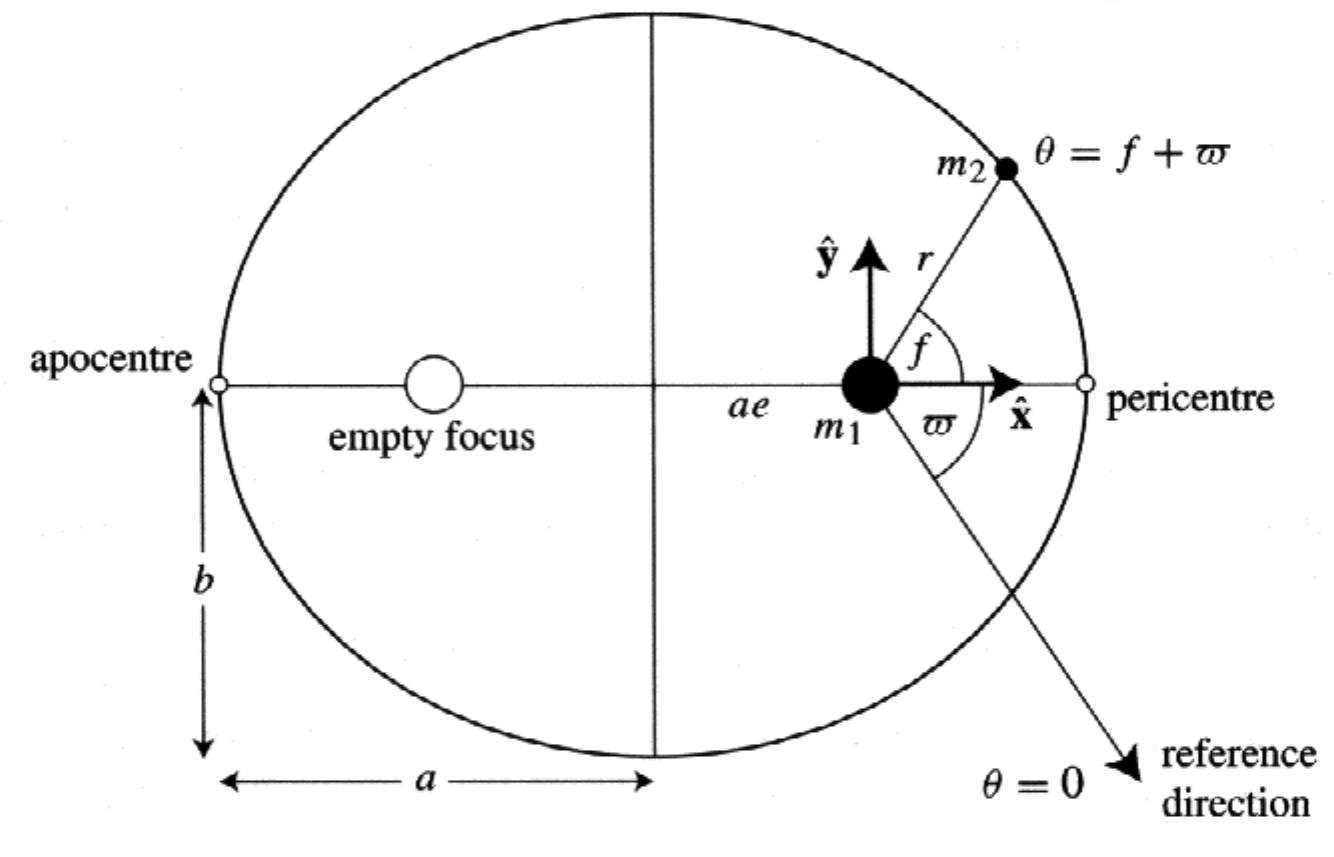
\includegraphics[width=\linewidth]{gfx/ellipse.png}
\caption{An elliptical orbit. The mass $m_1$ sits in one focus and $m_2$ orbits 
    around it. The postion of $m_2$ on the ellipse is specified by two angles, 
    the true anomaly $f$ and the argument of pericentre $\omega$. Only $f$ 
    varies in the two--body problem, $\omega$ stays fixed in the absence of an
    external perturbation. Figure taken from \citet{murray}.}
\label{fig:ellipse}
\end{figure}
\Cref{fig:ellipse} shows an elliptical orbit in two dimensional space. The mass
$m_2$ orbits around $m_1$ which is located in one of the focci of the ellipse.
The position of $m_2$ at each moment in time is described by the $2\pi$-periodic
angle 
$f=\theta - omega$ called the \emph{true anomaly}. The angle $\omega$ is specified 
relative to an arbitrary reference direction and it is constant throughout the 
motion. $f=0$ corresponds to the closest approach of $m_2$ to $m_1$, this point on
orbit is called the \emph{pericentre}. Conversely, the point furthest away from 
$m_2$ at $f=\pi$ is called the \emph{apocentre} . 
The \emph{semi-major axis} of the ellipse $a$ is given by
\begin{equation}
    a= \frac{h^2}{\mu} \frac{1+e}{1-e} 
\end{equation}
One can easily derive \citep[ex.][]{murray} \emph{Kepler's third law} which says 
that
\begin{equation}
    T^2= \frac{4\pi^2}{\mu} a^3
    \label{eq:kepler_law}
\end{equation}
where $T$ is the orbital period of $m_2$ around $m_1$. We also define the so-called
\emph{mean motion} $n$, as
\begin{equation}
    n= \frac{2\pi}{T} 
\end{equation}
The mean motion is the average angular frequency of the periodic motion. It is 
constant in the two--body problem but in general varies when additional bodies are 
present.

If we multiply \cref{eq:4} by $\dot{\vect{r}}$ and use the expressions for
$\dot{\vect{r}}$ and $\ddot{\vect{r}}$ from \cref{eq:9}, we obtain the following
constant of motion
\begin{equation}
    \frac{1}{2} v^2 - \frac{\mu}{r} =C
\end{equation}
where $v^2=\dot{\vect{r}}\cdot\dot{\vect{r}}$ is velocity squared and $C$ is a
constant of motion, the energy per unit mass. It can be shown \citep{murray}
that $C$ is given by
\begin{equation}
    C= -\frac{\mu}{2a} 
\end{equation}
thus, of a closed orbit in the two--body problem depends only on the semi-major axis.
\subsection{The mean and eccentric anomaly}
By solving the orbit equation, we have established that the mass $m_2$ orbits 
around $m_1$ in an ellipse if $e<1$. However, it is not immediately clear how
to explicitly solve for the time dependance of $r$ and $f$ and thus determine 
the position of $m_2$ at any given time. It is obvious that $f$ and $r$ vary
non-linearly with time for $e\neq 0$. For reasons which will become apparent 
later, we would like to construct an angle which varies linearly with time.
One such angle is the \emph{mean anomaly} $M$ defined as
\begin{equation}
    M=n(t-\tau)
\label{eq:mean_anomaly}
\end{equation}
where $\tau$ is the \emph{time of pericentre passage} and is constant. $M$
incrases linearly with time at a rate equal to the mean motion. At $t=\tau$ 
we have $M=f=0$
and at $t=\tau + T/2$ $M=f=\pi$, thus at the pericentre and apocentre 
M matches with $f$. The angle $M$ has no obvious geometricall significance
but we can define another angle which does. \Cref{fig:eccentric_anomaly} 
shows the orbital ellipse with semi-major axis $a$ together with a 
circumscribed circle of radius $a$ concentric with the ellipse. A line 
perpendicular to the semi-major axis of the ellipse interesects two points,
one on the orbit and one on the circumscribed circle. We define the 
\emph{eccentric anomaly} $E$ to be the angle between the semi-major axis
of the ellipse and the intersected point on the circle. Again, we have
$E=M=0$ at $f=0$ and $E=M=\pi$ at $f=\pi$. 
\begin{figure}[htb]
\centering
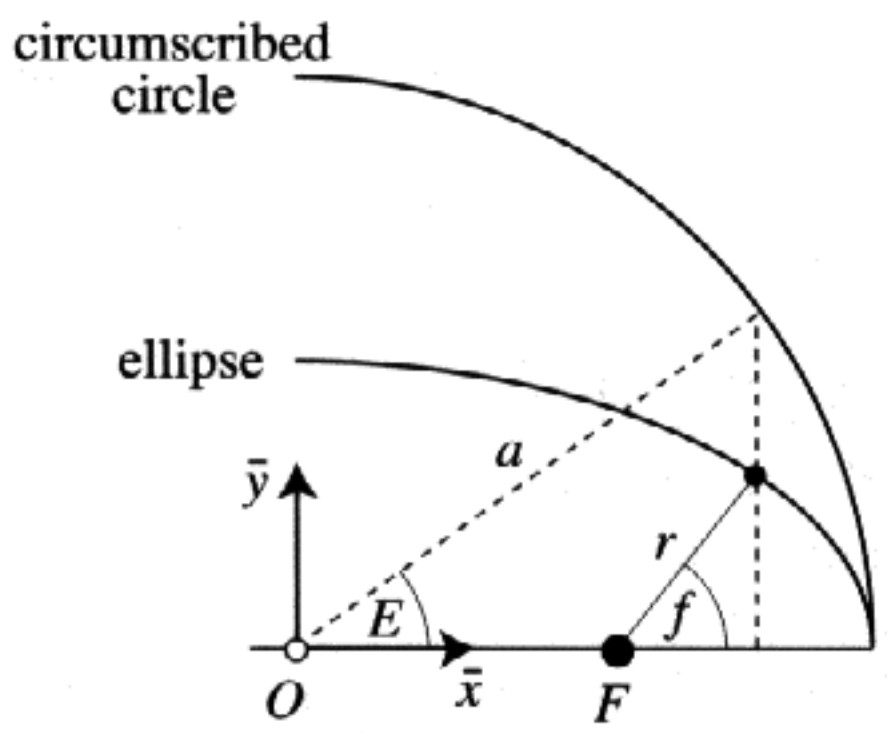
\includegraphics[width=0.5\linewidth]{gfx/eccentric_anomaly.png}
\caption{A geometrical description of the eccentric anomaly $E$.}
\label{fig:eccentric_anomaly}
\end{figure}
From geometry one can show that the following relation between the
angles $f$ and $E$ is satisfied
\begin{equation}
    \cos f= \frac{\cos E -e}{1-e\cos E} 
    \label{eq:eccentric_anomaly}
\end{equation}
Thus, there is a one-to-one correspondance between $f$ and $E$. To 
locate the location of the body on its orbit at time $t$, we need
a relationship between $E$ and $M$. This relation ship is called
the \emph{Kepler's equation} and is given by \citep{murray}
\begin{equation}
    M=E-e\sin E
    \label{eq:kepler_equation}
\end{equation}
A solution to this equation enables us to locate the body on its orbit
at any given time. The procedure is as follows
\begin{enumerate}
    \item At a particular time $t$ find $M$ from \cref{eq:mean_anomaly}
    \item Solve the Kepler's equation for $E$
    \item Use \cref{eq:eccentric_anomaly} to find $f$
\end{enumerate}
Kepler's equation is transcendental in $E$ and therefore it cannot
be solved directly. 

Finally, we define one last angle $\lambda$ called the
\emph{mean longitude} as
\begin{equation}
    \lambda =M +\omega
\end{equation}
Since it is derived from $M$, it does not have a geometrical 
interpretation. All longitudes are defined with respect to a 
common, arbitrary reference point.
\subsection{Orbit in an inertial frame}
So far we have derived a solution for the \emph{relative} motion
of $m_2$ with respect to $m_1$, we now turn to the description of the
orbit in a non-accelerating \emph{inertial frame}.
\begin{figure}[htb]
\centering
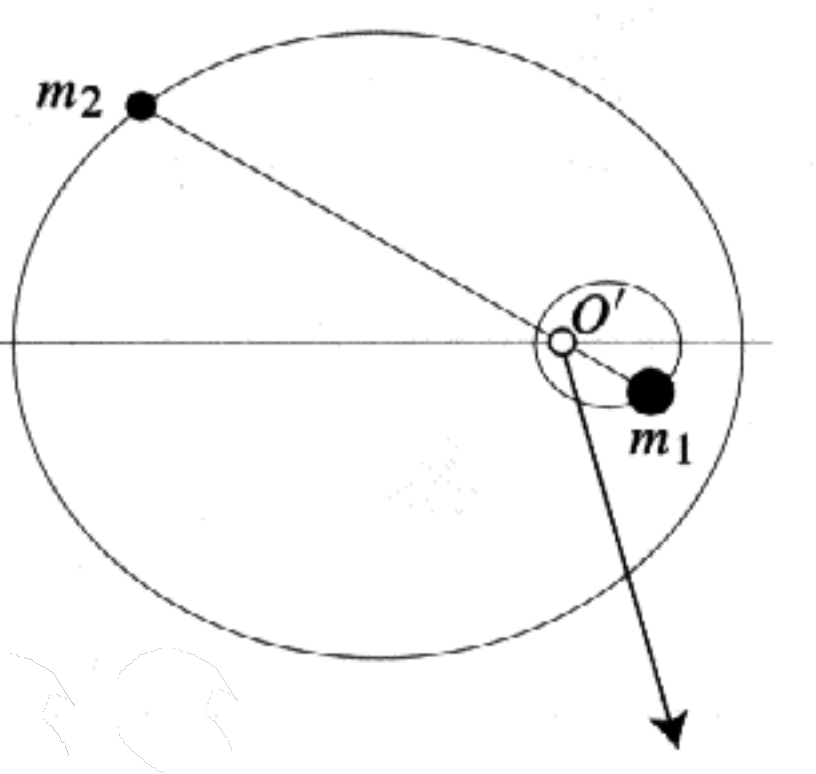
\includegraphics[width=0.5\linewidth]{gfx/barycentric_orbit.png}
\caption{The motion of $m_2$ and $m_1$ with respect to their centre
    of mass $O'$.}
\label{fig:barycentric_orbit}
\end{figure}
It is not difficult to show that the the masses $m_1$ and $m_2$ again
orbit in a conic section around their centre of mass with the same
period $T$ as before. 
\Cref{fig:barycentric_orbit} shows the orbits with respect to the
centre of mass. We need not worry about the motion of the centre
of mass itself because of a result from elementary mechanics which says
that the centre of mass of a collection of particles always moves at
constant velocity in a straight line and is therefore a valid inertial
reference frame. The conic sections of the orbits relative to the centre
of mass are 
reduced in scale by mass factors, as follows
\begin{equation}
    a_1= \frac{m_2}{m_1 + m_2} a\quad a_2= \frac{m_1}{m_1 + m_2} a
\end{equation}
where $a_1$ is the semi-major axis of the orbit of $m_1$ around $O'$
and $a_2$ is the semi-major axis of the orbit of $m_2$ around $O'$.

The \emph{total} angular momentum of the system is given by 
\begin{equation}
    L= \frac{m_1 m_2}{m_1 + m_2} \sqrt{\mu a(1-e^2)}
    \label{eq:ang_momentum}
\end{equation}
and the total orbital energy is
\begin{equation}
    E= -G \frac{m_1 m_2}{2a} 
\end{equation}
The energy of a Keplerian orbit depends only on the semi-major axis
and the angular momentum depends on both the semi-major axis and
the eccentricity. In particular, if the semi-major axis is constant
the only way to change the eccentricity is by changing the angular
momentum. This simple fact is the essence of so-called secular
interactions described in \cref{sec:three_body}. The angular momentum
is largest for a circular orbit.

\subsection{Orbit in three-dimensional space}
We have determined that the bodies in the two--body problem move on
on an ellipse in inertial space. The orientation of that ellipse 
stays fixed for all time if no external bodies are present. If there 
are also other bodies in the system however, the orbit no longer stays
fixed, both its shape and orientation change in three-dimensional space.
Because of that it is useful to define the orientation of the orbit
in 3D space relative to a fixed reference plane.
\begin{figure}[htb]
\centering
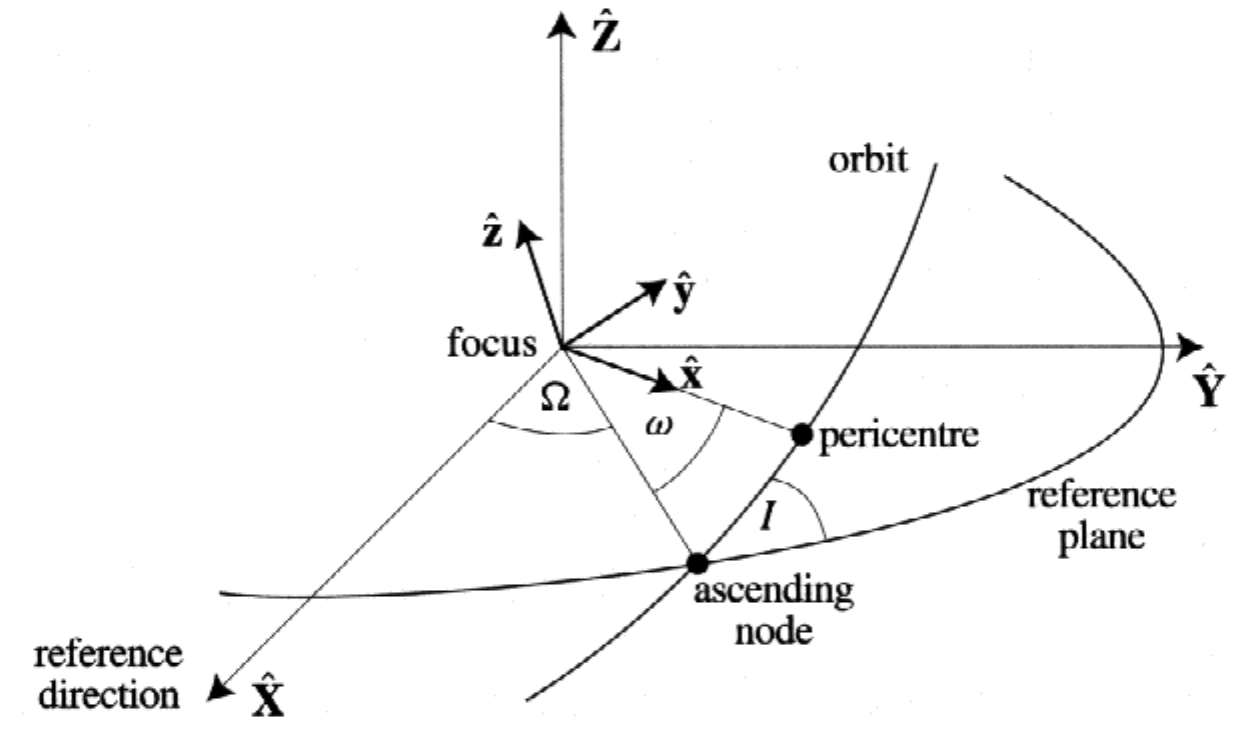
\includegraphics[width=0.8\linewidth]{gfx/3d_orbit.png}
\caption{A keplerian orbit in 3D space.}
\label{fig:3d_orbit}
\end{figure}
\Cref{fig:3d_orbit} shows the orbit in 3D Cartesian coordinate system,
the reference plane is taken to be the $X-Y$ plane. The orbital
ellipse intersects the reference plane in two point. In order to define
its orientation relative to fixed axes we have to choose one. Independent
on wheater the orbiting body is moving around the ellipse in a clockwise
or counter-clockwise direction, the body will pass through the reference
plane \emph{from below} (where below is the $-Z$ direction)
at one of the two points. We call this point the \emph{ascending node}
and choose it as a reference. The angle from the ascending node to the
$X$ axis is then called the \emph{longitude of the ascending node} and
is denoted by $\Omega$. The angle between the plane of the ellipse and
the reference plane is called the \emph{inclination} of the orbit and
is defined in the range $0\leq I\leq \pi$.
Thus, we have completely described the orbit in 3D space. However, it is useful to 
define another angle $\varpi$ called the \emph{longitude of pericentre.} 
$\varpi$ is not really a true angle since it is defined as a sum of 
angles in two seperate planes. When the inclination is zero (the orbit
is co-planar with the reference plane) $\varpi=\omega$. 

It can be shown that each there is a one-to-one correspondance between 
a set of Cartesian positions and velocities $(x,y,z,v_x,v_y,v_z)$ 
of a given massive particle and an \emph{instantaneous} Keplerian orbit 
defined by $(a,e,I,\Omega,\omega,f)$ with respect to another massive
particle. This why it is still usefull to talk about orbits even
when we are dealing with a system of multiple bodies. Altough those
bodies won't stay on a fixed Keplerian orbit for all time, at any given
time we can still define an instantaneous Keplerian orbit.

Most bodies in stable systems change their orbital elements slowly
when exchanging energy and angular momentum with other bodies, thus
it is often more useful to use the orbital elements as a set of coordinates
instead of the Cartesian coordinates.

\section{A brief review of Hamiltonian mechanics}
\label{sec:hamiltonian_mechanics}
\subsection{Hamilton's equations}
\label{sub:Hamilton's equations}
The two--body prolem could have been solved equally well using a different
formulation of mechanics called \emph{Hamiltonian mechanics} after
William Rowan Hamilton (1805-1865). Hamiltonian
mechanics is equivalent to Newtonian mechanics but is often more suitable
for certain types of problems and the concept of a Hamiltonian function
is a lot more general than Newton's second law of mechanics.

In Newtonian mechanics the full description of a dynamical system 
consisting of N particles is 
obtained by solving a system of second order differential equations
of the form
\begin{equation}
    \dot{\vect{p}}_i=\vect{F}_i
\end{equation}
where $\dot{\vect{p}}_i=m_i\dot{\vect{r}}_i$ is the momentum of the
i-th particle, $m_i$ is its mass and $\vect{r}_i$ its position vector
relative to an origin of an inertial reference system. This 
constitutes a system of 3N second order differential equations for
the positions vectors $\vect{r}_i$.

In the Hamiltonian formalism a dynamical system is described by 
a function of \emph{generalized coordinates} $\vect{q}$ and \emph{momenta} 
$\vect{p}$ called the \emph{Hamiltonian} $\mathcal{H}(\vect{q},
\vect{p})$. Each pair $(q_i,p_i)$ constitutes a single 
\emph{degree of freedom}, it is said to be \emph{conjugate} . 
The time evolution of these coordinates and 
momenta
$(\vect{q},\vect{p})$, collectively known as the \emph{phase space} 
is given by \emph{Hamilton's equations} 
\begin{equation}
    \dot{q}_i= \frac{\partial \mathcal{H}}{\partial p_i}\quad
    \dot{p}_i= \frac{\partial \mathcal{H}}{\partial q_i} 
    \label{eq:hamiltons_equations}
\end{equation}
Instead of 3N second order differential equations for a system of N particles
, we now have 
6N \emph{coupled first-ordered} equations. Once the initial conditions
$(\vect{q}_0,\vect{p}_0)$ are specified, the solution of Hamilton's 
equations defines a \emph{unique} trajectory in a 
6N dimensional phase space. The coordinate pair $(\vect{q},\vect{p})$
is said to be \emph{canonical} if the coordinates satisfy 
Hamilton's equations. The main advantage of the Hamiltonian
formalism compared to other formalisms of mechanics is the ability
to easily transform to different choices of $(\vect{q},\vect{p})$
as long as the new set of coordinates is also canonical. There are no
other strict requirements on the new coordinates, the momentum 
$p_i$ coincides with the real momentum $m_i \dot{q_i}$ only in
Cartesian coordinates.

We can arbitrarily scale the momentum and the coordinate by a 
constant factor, for example $p\rightarrow\eta p\quad q\rightarrow\nu q$, 
, as long as we also
rescale the time. This is obvious from the form of 
\cref{eq:hamiltons_equations} because
\begin{equation}
    \frac{\partial \mathcal{H}}{\partial (\eta p)}= 
    \frac{\mathrm{d}q}{\mathrm{d}(\eta t)}  
    \label{eq:rescaling_hamiltonian}
\end{equation}
and similary for the coordinate scaling. Transformations of this
type are known as \emph{scale transformations} and they are simply 
a reflection of the fact that the equations of motion should be invariant
to the changes of units.
\subsection{Integrable Hamiltonians}
The Hamiltonian formalism is useful for finding conserved quantities.
If a generalized coordinate $q_i$ does not appear in the Hamiltonian
the the corresponding momentum conjugate $p_i$ is a conserved quantity
\begin{equation}
    \dot{p}_i= \frac{\partial \mathcal{H}}{\partial q_i} =0
\end{equation}
If the motion is in a fixed potential, the Hamiltonian is equal
to the total energy of the system $E$.

If a particular hamiltonian $\mathcal{H}$ can be reduced to a form
where it depends only on the momenta, that is
\begin{equation}
    \mathcal{H}(\vect{p})
\end{equation}
then the momenta $\vect{p}$ are conserved and the system is said to be
\emph{integrable}. An integrable system with $n$ degrees of freedom
has $n$ constants of motion. From Hamilton's equations, it follows that the time
evolution of the coordinates is simply
\begin{equation}
    \dot{q}_i= \frac{\partial \mathcal{H}}{\partial p_i} =\omega_i
\end{equation}
that is, all of the coordinates evolve linearly in time with constant
frequencies $\omega_i$ which depend only on the momenta
\begin{equation}
q_i(t)=\omega_i t
\end{equation}
Integrable system are very rare and it is not immediately clear
if a given Hamiltonian can be reduced to an integrable form.

Systems of the form
\begin{equation}
    \mathcal{H}=\mathcal{H}_0(\vect{p})+\epsilon \mathcal{H}_1(\vect{q})
\end{equation}
where $\mathcal{H}_0$ is an integrable Hamiltonian, $\mathcal{H}_0$ is 
a perturbation and $\epsilon$ is a small parameter are said to be nearly 
integrable
and in general they display chaotic behaviour .However, if $\epsilon$ is 
small enough most solutions still lie in the region of phase space
allowed by the solutions of $\mathcal{H}_0$.

Systems with a single degree of freedom are always integrable and
the Hamiltonian itself is a conserved quantity (i.e. the energy
is conserved). The trajectory is defined completely by the value
of energy. They are often used as an approximation for a generally
more complex system. Obtaining a single degree of freedom
Hamiltonian for a resonance is a major goal in 
\cref{ch:analytical_model_of_high_order_mmrs}.

The Keplerian Hamiltonian for the two--body problem is completely 
integrable. It can be written as
\begin{equation}
    \mathcal{H}_k=- \frac{\mu^2\mu^*}{2\Lambda^2} 
\end{equation}
where $\mu^*=m_1m_2/(m_1+m_2)$ and $\Lambda$ is the generalized
momentum conjugate to the orbital element coordinate $\lambda$,
the mean anomaly. The original Keplerian Hamiltonian has 6 
degrees of freedom, the conservation of total linear and total
angular momentum vectors and the conservation of total energy
give 7 constants of motion. There is also a hidden symmetry in
the problem that we haven't mentioned. One can show that
one of the three components of the 
\emph{Runge-Lenz} vector is also a constant of motion, which 
bring the total to 8. The Runge-Lenz vector is a vector pointing
in the direction of periastron, defined by
\begin{equation}
    \vect{e}=\dot{\vect{r}}\times(\vect{r}\times\dot{\vect{r}})
    /(G(m_1+m_2)) - \vect{\hat r}
\end{equation}
Its magnitude is equal to the eccentricity of the orbit. We 
see that the number of constants of motion over-determines the 
problem. In fact, the two extra constants of motion are responsible
for the fact that that the relative motion is not only restricted to 
a conic curve but it is also a conic section in the inertial
(centre of mass) frame. Due to this fact the orbit is also fixed in
3D space.

\subsection{Fixed points}
Given a Hamiltonian $\mathcal{H}(q,p)$ with a single degree of freedom
its \emph{fixed points} are solutions of
\begin{equation}
    \dot{p}=0\quad\dot{q}=0
\end{equation}
Those are points at which there is no motion in phase space. From 
Hamilton's equations, it follows that their location is given by
\begin{equation}
   \frac{\partial \mathcal{H}}{\partial p}= \frac{\partial \mathcal{H}}{\partial q}=0
\end{equation}
Given a fixed point $(q_0,p_0)$, we would like to derive the equations
of motion in its vicinity. If a test particle in its vicinity moves 
on a trajectory away from the fixed point, the point is said to be
\emph{unstable}. Conversely, if it remains near the fixed point for all 
time, the point is said to be \emph{stable}. We can expand the Hamiltonian
near the fixed point in a Taylor series
\begin{align}
    \mathcal{H}(\tilde q, \tilde p)=\mathcal{H}(q_0,p_0) 
    + \frac{\partial^2\mathcal{H}(q_0,p_0)}{\partial q^2} \frac{\tilde q^2}{2} 
    &+\frac{\partial^2\mathcal{H}(q_0,p_0)}{\partial p^2} \frac{\tilde p^2}{2} \nonumber\\
    &+\frac{\partial^2\mathcal{H}(q_0,p_0)}{\partial q\partial p}\tilde q\tilde p 
\end{align}
where $\tilde q=q-q_0$ and $\tilde p=p-p_0$. We can write this more succinctly 
in vectorial form as
\begin{equation}
    \mathcal{H}(\tilde q,\tilde p)= \frac{1}{2} \vect{x}^\tau\vect{M}\vect{x}
\end{equation}
where $\vect{x}=(\tilde q, \tilde p)$ and $\tau$ denotes the transpose 
operation. $\vect{M}$ is called the \emph{Hessian matrix} and is given by
\begin{equation}
    \vect{M}=
    \begin{pmatrix}
        \frac{\partial^2 \mathcal{H}}{\partial q^2} &
        \frac{\partial^2 \mathcal{H}}{\partial q\partial p }\\
        \frac{\partial^2 \mathcal{H}}{\partial p \partial q} &
        \frac{\partial^2 \mathcal{H}}{\partial p^2} 
    \end{pmatrix}
    \label{eq:fixed_points_stability}
\end{equation}
The matrix $\vect{M}$ is evaluated at the fixed points $(q_0,p_0)$.
It is symmetric which means that it has two real 
eigenvalues and two eigenvectors. It can be shown that after 
diagonalizing this matrix, the Hamiltonian assumes the form
\begin{equation}
    \mathcal{H}(q,p)= \frac{1}{2} (\lambda_1 q^2 + \lambda_2 p^2)
\end{equation}
where $\lambda_1$ and $\lambda_2$ are the eigenvalues. If the
eigenvalues are both negative or both positive (i.e. the
determinant is positive) the system undergoes
harmonic oscillations (librations) about the fixed point with 
frequency
\begin{equation}
    \omega = \sqrt{\lambda_1\lambda_2}
\end{equation}
and we say the fixed point is a \emph{center}. If one of the 
eigenvalues is negative and the other positive (the determinant
is negative) the system is
diverging exponentially away from the fixed point in the 
direction of one \emph{eigenvector} and heading towards the 
fixed point along the direction of the other eigenvector. The
fixed point is unstable and we call it a \emph{saddle} .

\subsection{Canonical transformations}
\label{sub:Canonical transformations}
A \emph{canonical transormation} is a coordinate transformation
from a set $(\vect{q},\vect{p})$ to $(Q(\vect{q},\vect{p}),
P(\vect{q},\vect{p})$ which preserves the form of Hamilton's
equations. It can be shown that canonical transformations
satisfy the Poisson brackets
\begin{equation}
    \{P_i,P_j\}=0\quad\{Q_i,Q_j\}=0\quad\{Q_i,P_j\}=\delta_{i,j}
\end{equation}
where $\delta_{i,j}$ is the \emph{Kronecker delta} symbol and
the Poisson bracket is defined as
\begin{equation}
    \{f,g\}=\sum^N_{i=0}\left( \frac{\partial f}{\partial q_i} 
    \frac{\partial g}{\partial p_i} -\frac{\partial f}{\partial p_i} 
    \frac{\partial g}{\partial q_i} \right)
\end{equation}
where the sum goes over all the degrees of freedom. The question now
is how to easily construct transformations which are canonical. The
answer lies in the form of \emph{generating functions}. Consider
a function $F_1(q,Q)$ of the old and new coordinates and let
\begin{equation}
    p_i= \frac{\partial F_1}{\partial q_i} 
\end{equation}
After inverting, this equation defines a new coordinate $Q_i=Q_i(q,p)$.
One can show that the new momentum is then given by
\begin{equation}
    P_i=- \frac{\partial F_1}{\partial Q_i} 
\end{equation}
Thus we have found a way to construct a canonical transformation to new
coordinates. We choose the new coordinates $Q_i$, however, the requirement 
that the new coordinates form a conjugate pair restricts are freedom
to choose the new momentum as well. The function $F_1(q,Q)$ is called
the \emph{generating function of first kind} . There are three additional
kinds of generating functions, the possibilities are listed in 
\cref{tab:generating_functions}.
\begin{table}[h!]
\centering
\begin{tabular}{cll}
\toprule
    Generating function &\multicolumn{2}{c}{Derivatives}\\
\midrule
    $F_1(q,Q)$ & $p_i=\frac{\partial F_1}{\partial Q_i}$ & 
    $P_i=\frac{\partial F_1}{\partial q_i}$\\
    $F_2(q,P)$ & $p_i=\frac{\partial F_2}{\partial q_i}$ & 
    $Q_i=\frac{\partial F_2}{\partial P_i}$\\
    $F_3(p,Q)$ & $q_i=-\frac{\partial F_3}{\partial p_i}$ & 
    $P_i=-\frac{\partial F_3}{\partial Q_i}$\\
    $F_4(p,P)$ & $q_i=-\frac{\partial F_4}{\partial p_i}$ & 
    $Q_i=\frac{\partial F_4}{\partial P_i}$\\
\bottomrule
\end{tabular}
\caption{Different kinds of generating functions.}
\label{tab:generating_functions}
\end{table}
Which kind of the generating function is the best depends on the
problem at hand.

\section{The pendulum}
\label{sec:pendulum}
A simple single degree of freedom Hamiltonian useful for the study
of resonance is that of the pendulum. The Hamiltonian has the form
\begin{equation}
    \mathcal{H}(\phi,p)= \frac{1}{2} p^2 -\omega_0^2\cos\phi
\end{equation}
Where $\omega_0$ is the frequency of oscillations. By solving 
Hamilton's equations, we obtain
\begin{align}
    \dot{\phi} &= p\\
    \dot{p} &= - \omega_0^2\sin\phi
\end{align}
Combining the two equations, we obtain a single equation of motion
\begin{equation}
    \ddot{\phi}+\omega_0^2\sin\phi =0
\end{equation}
We see that in the limit of small $\phi$ the motion is equivalent to
that of the harmonic oscillator oscillating with the frequency
$\omega_0$. The fixed points are located at
$(\phi, p)=(\pm k\pi,0)$ (where k is an interger) and there is 
a single 
stable center point located at $(\phi¸ p)=(\pi, 0)$. It is 
sufficient to study the two fixed points $(0,0)$ and $(\pi,0)$
since the motion is periodic. For the fixed point at $(0,0)$, we have
\begin{equation}
    \vect{M}=
    \begin{pmatrix}
        0 & 1\\
        -1 & 0
    \end{pmatrix}
\end{equation}
and we see that this point is a stable center. For the other point 
at $(\pi,0)$, we have
\begin{equation}
    \vect{M}=
    \begin{pmatrix}
        0 & 1\\
        1 & 0
    \end{pmatrix}
\end{equation}
The point is a an unstable saddle point.
\begin{figure}[htb]
\centering
\includegraphics[width=\linewidth]{gfx/pendulum.pdf}
\caption{The phase space of a pendulum. There red curve denotes the 
    separatrix filled circles denote stable fixed points, open circles denote
    unstable fixed points.}
\label{fig:pendulum}
\end{figure}
\Cref{fig:pendulum} shows the level curves (curves of constant $\mathcal{H}$)
of the pendulum. Given a specific value of the energy, the system stays 
on one of the curves for all time. The motion around the fixed point $(0,0)$
 in between the fixed points at $-\pi$ and $\pi$ is said to be \emph{libratory}.
There is also an entirely different type of motion where $\phi$ is unbounded,
these trajectories are called \emph{circulatory}. The curve which passes through
the unstable points separates the two regimes and is called the \emph{separatrix.} 
As seen from the figure\footnote{This can also be shown rigorously by deriving the
expression for $\omega_{lib}$ as a function of maximum $\phi$.},
the oscillation period increases from the initial
small amplitude value of $2\pi/\omega_0$ to infinity as the separatrix is
approached. Once the separatrix is crossed the motion is unbounded. This
steep dependance of the librational period on the distance to the separatrix is
responsible for chaos in weakly interacting non-linear systems. The concepts
presented in this section will be important for the study of resonance in the
three--body problem.

\section{The three--body problem}
\label{sec:three_body}
\subsection{The disturbing function}
Finally, we move to the problem of three gravitationally interacting massive 
bodies suchs as the circumbinary system consisting of two stars and 
an outer planet. The three--body problem is famously not integrable, many 
great mathematicians such as Newton and Poincaré have tried and failed to find and
exact solution. However, it is still possible to do a perturbative analysis
in the case when one of the bodies is only weakly interacting with the
other two. The following discussion largely follows \citet{Mardling2013}.

A stable hierarchical system of three bodies naturally divides into
two orbits composed of an "inner binary" and an "outer binary". We will work
in \emph{Jacobi coordinates} which are defined such that in a hierarchical
system consisting of $N$ bodies, the $N$th body is defined in a coordinate 
system whose origin is the centre of mass of the previous $N-1$ bodies. 
\Cref{fig:jacobi} shows a system of three masses $m_1$, $m_2$ and $m_3$ in
Jacobi coordinates. The position vector $\vect{r}$ points from $m_1$ to $m_2$ 
and it is the same vector as in our previous analysis of the two--body 
problem. The position vector $\vect{R}$ points from the centre of mass
of the inner binary consisting of $m_1$ and $m_2$ to the outer mass $m_3$.
Thus, at any given moment we can define two Keplerian orbits, one for
the inner binary and one for the outer binary. Since the three--body
problem is not integrable the orbits will in general no longer be fixed
and will change their orbital elements with time. This choice of coordinates
obviously fails in the case of crossing orbits since the hiararchy loses
its meaning, however, a system with crossing orbits is inherently unstable
and not the subject of our interests.
\begin{figure}[htb]
\centering
\includegraphics[width=\linewidth]{gfx/jacobi.pdf}
    \caption{A system of three massive bodies in Jacobi coordinates. 
    The point $C_{12}$ denotes the centre of mass of the inner two 
    bodies and the point $C_{123}$ that of the whole system.}
\label{fig:jacobi}
\end{figure}

When the system is stable the inner and outer orbits interact only 
weakly by means of an interacting potential called the 
\emph{disturbing function}. The disturbing function can be written
as an infinite Fourier series of angles called the \emph{resonance
angles}, it is responsible for the exchange of energy and angular 
momentum between the two orbits.  Each resonance angle is a linear
superposition of all angles in the system. A resonance angles can either 
circulate or librate in exactly the same way as in the pendulum model
described in the previous section.
If a particular resonance angle is librating, we say that the system
is in \emph{resonance}. The various resonance angles can mutually 
interact, under certain conditions a system can exisist in two 
neighbouring resonant states where two resonant angles librate 
at a similar period. This is known as \emph{resonance overlap} 
and it leads to chaotic behaviour as the resonance angle approaches
the unstable fixed points \citep{WalkerFord1969}. The resonance
overlap criterion is then a good indication of wheather the
system is stable or not.

We can write the equations of motions as
\begin{equation}
\begin{aligned}
    m_1\ddot{\vect{r}}_1&= \frac{Gm_1m_2}{r^2_{12}} \vect{\hat r}_{12}+
    \frac{Gm_1m_3}{r^2_{13}} \vect{\hat r}_{13}\\
    m_2\ddot{\vect{r}}_2&= -\frac{Gm_1m_2}{r^2_{12}} \vect{\hat r}_{12}+
    \frac{Gm_2m_3}{r^2_{23}} \vect{\hat r}_{23}\\
    m_3\ddot{\vect{r}}_3&= -\frac{Gm_1m_3}{r^2_{13}} \vect{\hat r}_{13}-
    \frac{Gm_2m_3}{r^2_{23}} \vect{\hat r}_{23}
\label{eq:three_body_newton}
\end{aligned}
\end{equation}
where the position vectors $r_i$ point from the centre of mass of 
system $C_{123}$ to the mass $m_i$ and $\vect{r}_{ij}=\vect{r}_j-\vect{r}_i$. 
\Cref{eq:three_body_newton} constitues a system with 9 degrees of freedom.
Again we have the 7 conserved quantities due to momentum and energy 
conservation, however, there is no analogue of the Runge-Lenz vector
in the three--body problem. Therefore, the system is not completely
integrable, in fact, it admits \emph{chaotic} solutions -- solutions which
are extremely sensitive to small variations in the inital conditions. 
There are two kinds of stability. One is called \emph{Lagrange stability} 
and the other \emph{Hill instability}. The latter happens due to close
approaches of two bodies, the former does not require close approaches.
In this chapter we are primarily interested in Lagrange instability 
since scattering events are difficult to handle analytically
and only become important after the onset of Lagrange instability in 
circumbinary systems, because the circumbinary planet is initally far away
from the inner stellar binary.

We start by rewriting \cref{eq:three_body_newton} in Jacobi coordinates
and define the vectors $\vect{r}=\vect{r}_2-\vect{r}_1$ and 
$\vect{R}= (m_{123}/m_{12})\vect{r}_3$ 
where $\vect{r}$ is the same relative position vector from the two--body 
problem and $\vect{R}$ points from the centre of mass $C_{12}$ to $m_3$.
We can now rewrite \cref{eq:three_body_newton} as
\begin{align}
    \mu_i\ddot{\vect{r}}+ \frac{Gm_1m_2}{r^2} \vect{\hat r}&= \frac{
        \partial \mathcal{R}}{\partial \vect{r}} \\
    \mu_o\ddot{\vect{R}}+ \frac{Gm_{12}m_3}{R^2} \vect{\hat R}&= \frac{
        \partial \mathcal{R}}{\partial \vect{R}} 
    \label{eq:three_body_newton_R}
\end{align}
where $R=\lvert\vect{R}\rvert$, $\mu_i=m_1m_2/m_{12}$ and $\mu_o=m_{12}m_3/m_{123}$
and
\begin{equation}
    \mathcal{R}=- \frac{Gm_{12}m_3}{R} + \frac{Gm_2m_3}{\lvert\vect{R}-\beta_1\vect{r}
    \rvert} + \frac{Gm_1m_3}{\lvert\vect{R}+\beta_2\vect{r}\rvert}
    \label{eq:dist_cartesian}
\end{equation}
is the disturbing function with $\beta_i=m_i/m_{12},\,i=1,2$. We use the subscripts
$i$ and $o$ to denote quantities defined with respoct to the inner and outer orbits
respectively. The notation $\partial/\partial\vect{r}$ refers to the gradient with 
respect to the spherical polar coordinates $(r,\theta_1,\phi_1)$ 
associated with the position od body 2 relative to the centre of mass $C_{12}$, similarly,
$\partial/\partial\vect{R}$ for the position of body 3 with coordinates $(R,\theta_o,\phi_o)$
relative to the same origin. All information
about the mutual interaction of the inner and outer orbits is contained in
$\mathcal{R}$\footnote{Historically, most versions of the expanded disturbing
function have units of energy per unit mass. The expansion presented in RM2013 has
units of energy}. In the limit when the inner two masses coalesce ($r/R\rightarrow 0$)
or the mass ratio between the planet mass $m_3$ and the total binary mass $m_{12}$
goes to zero ($m_3/m{12}\rightarrow 0$) $\mathcal{R}$ vanishes and the two orbits
no longer interact with each other. The total energy (or the Hamiltonian) is given by
\begin{equation}
    \mathcal{H}=\mathcal{H}_i+\mathcal{H}_o-\mathcal{R}
    \label{eq:three_body_hamiltonian}
\end{equation}
where
\begin{equation}
    \mathcal{H}_i= \frac{1}{2}\mu_i\dot{\vect{r}}\cdot\dot{\vect{r}}- \frac{Gm_1m_2}{r}, \quad
    \mathcal{H}_o= \frac{1}{2}\mu_o\dot{\vect{R}}\cdot\dot{\vect{R}}- \frac{Gm_{12}m_3}{R}
\end{equation}
are the Keplerian Hamiltonians corresponding to the inner and outer orbits and the 
disturbing function has a role of interaction energy. The two Keplerian Hamiltonians
individually are fully integrable as mentioned previously, the complete Hamiltonian
is not. 

Given 
\cref{eq:three_body_hamiltonian}, one can calculate the Hamilton's equations of
motion. Those are equivalent to \cref{eq:three_body_newton_R}, except that they
are first order in time. If those equations are are then expressed in terms
of the inner and outer orbital elements, they are called 
\emph{Lagrange's planetary equations}. The derivation is presented
in \cite[ex.][]{brouwer1961}, here we merely state the result for coplanar
systems
\begin{equation}
\begin{aligned}
    \dot{e}&= -\frac{s(1-s)}{\mu na^2e} 
    \frac{\partial\mathcal{R}}{\partial\lambda}
    -\frac{s}{\mu na^2e} 
    \frac{\partial\mathcal{R}}{\partial\varpi}\\
    \dot{\varpi}&= \frac{s}{\mu na^2e} 
    \frac{\partial\mathcal{R}}{\partial e}\\
    \dot{\epsilon}&=- \frac{2}{\mu n a} 
    \frac{\partial\mathcal{R}}{\partial a}
   +\frac{s(1-s)}{\mu na^2e} 
    \frac{\partial\mathcal{R}}{\partial e} 
\end{aligned}
    \label{eq:lagrange_planetary_equations}
\end{equation}
where the subscripts of the orbital elements are either $i$
or $o$ for the inner and outer orbits respectively. $s=\sqrt{1-e^2}$
and $\epsilon$ is the mean longitude at $t=t_0$ and is related
to the mean longitude by $\int^t_0 n\mathrm{d}t$ 
\citep[see.][for details]{Mardling2013}. There is no unique general 
solution for \cref{eq:lagrange_planetary_equations}, best one can do
is to expand $\mathcal{R}$ in a series and consider a few dominant
terms in certain cases.

We start by expanding the last two terms in \cref{eq:dist_cartesian} using 
a well known\footnote{Expressions involving a difference between two vectors 
such as $1/\lvert \vect{r}-\vect{r}'\rvert$ occur in all kinds of problems 
in physics.} expansion in terms of \emph{spherical harmonics}. 
\begin{equation}
    \frac{1}{\lvert \vect{R} -\beta_s\vect{r}\rvert}= \frac{1}{R} \sum^\infty_{l=0}
  \frac{4\pi}{2l+1}   \left( \frac{\beta_s r}{R} \right)^l
    \sum^l_{m=-l} Y_{lm}(\theta_i,\phi_i)
    Y_{lm}^*(\theta_o,\phi_o)
    \label{eq:addition_theorem}
\end{equation}
$Y_{lm}$ is a spherical harmonic\footnote{Spherical harmonics are special
functions which form a complete set of orthogonal functions on the sphere, 
any function defined in terms of spherical polar coordinates can be expanded
in an infinite series of spherical harmonics as $f(\theta,\phi)
=\sum^\infty_{l=0}\sum^l_{m=-l}f^m_lY_l^m(\theta,\phi)$. The series converges 
if the coefficients $f^l_m$ decay in $l$ sufficiently rapidly.} of
\emph{degree l} and \emph{order m} with
$Y_{lm}^*$ being its complex conjugate. Using 
\cref{eq:addition_theorem} the disturbing function $\mathcal{R}$ becomes
\begin{equation}
    \mathcal{R}=G\mu_im_3\sum^\infty_{l=2}\sum^l_{m=-l}\left( \frac{4\pi}{2l+1} 
    \right)\mathcal{M}_l\left( \frac{r^l}{R^{l+1}} \right) Y_{lm}(\theta_i,\phi_i)
    Y_{lm}^*(\theta_o,\phi_o)
\label{eq:dist_harmonics}
\end{equation}
where $\mathcal{M}_l$ is a mass factor given by
\begin{equation}
    \mathcal{M}_l= \frac{m_1^{l-1}+(-1)^lm_2^{l-1}}{m_{12}^{l-1}} 
\end{equation}
\Cref{eq:dist_harmonics} is a spherical harmonic expansion with 
coefficients proportional to $(r/R)^l$. In order for this series
to converge, we require that $r/R$ is a small number. This is satisfied
for all circumbinary planets because as will be shown later, there is
an inner instability region outside of the stellar binary and the only
stable orbits exist further outside the stellar binary's orbit. A spherical
harmonic is defined by
\begin{equation}
    Y_{lm}(\theta,\phi)=\sqrt{ \frac{2l+1}{4\pi} \frac{(l-m)!}{(l+m)!} }\mathcal{P}_1^m(
    \cos\theta)e^{im\phi}
    \label{eq:sph_harmonics}
\end{equation}
where $\mathcal{P}_1^m(\theta, \phi)$ is the \emph{associated Legendre function}
\citep{jackson}. 

Next, we focus on coplanar systems
(mutual inclination between orbits is assumed to be zero) and thus we take
$\theta_i=\theta_o=\pi/2$ (the motion is restricted to the $x-y$ plane), 
$\phi_i=f_i+\varpi_i$ and $\phi_o=f_o+\varpi_o$ where $f_i$ and $f_o$ are
the true anomalies of the outer and inner orbits respectively. We obtain 
\begin{equation}
    \mathcal{R}=g\mu_im_3\sum^\infty_{l=2}\sum^l_{m=-l,2} \frac{1}{2} c_{lm}^2\mathcal{M}_l
    e^{im(\varpi_i-\varpi_o)}\left(r^le^{imf_i}\right)\left( \frac{e^{-imf_o}}{R^{l+1}} 
    \right)
    \label{eq:dist_expanded}
\end{equation}
where
\begin{equation}
    c^2_{lm}= \frac{8\pi}{2l+1} \left[Y_{lm}(\pi/2,0)\right]=c^2_{l-m}
\end{equation}
and the notation $m=-l, 2$ in the summation over $m$ means that the summation is taken
in steps of 2. The first few values for $c_{lm}$ can be found in \cite{Mardling2013}.
For stable systems the expressions in the last two brackets of
\cref{eq:dist_expanded} are nearly periodic and can therefore be expanded in a 
\emph{Fourier series} of the inner and outer mean anomalies $M_i=n_it+M_i(0)$ and
$M_o=n_ot+M_o(0)$, where $n_i,n_o$ are the mean motions associated with the inner
and outer orbits and $M_i(0),M_o(0)$ are their values at $t=0$.  The result is
\begin{equation}
    r^le^{imf_i}\stackrel{\mathcal{F}}{=}a_i^l\sum^\infty_{n=-\infty}X^{l,m}_n(e_i)e^{inM_i}
    \label{eq:expansion_1}
\end{equation}
and
\begin{equation}
    \frac{r^{-imf_o}}{R^{l+1}} \stackrel{\mathcal{F}}{=}a_o^{-(l+1)}\sum^\infty_{n'=-\infty}
    X^{-(l+1),m}_{n'}(e_o)e^{-n'M_o}
    \label{eq:expansion_2}
\end{equation}
where the $\mathcal{F}$ above the equality sign denotes Fourier expansion 
and the \emph{Fourier coefficients} are given by
\begin{equation}
    \begin{aligned}
        X^{l,m}_n(e_i)&= \frac{1}{2\pi} \int^{2\pi}_0 \left(\frac{r}{a_i}\right)^l
        e^{imf_i}e^{inM_i}\mathrm{d}M_i\\[4pt]
        &=\frac{1}{2\pi}\int^{2\pi}_0r^{l+1} e^{imf_i}e^{-inM_i}\mathrm{d}E_i
=    \mathcal{O}(e_i^{\lvert m-n\rvert})
    \label{eq:hansen_inner}
    \end{aligned}
\end{equation}
and
\begin{equation}
    \begin{aligned}
        X^{-(l+1),m}_{n'}(e_o)&= \frac{1}{2\pi} \int^{2\pi}_0 \left( \frac{R}{a_o}
        \right)^{-(l+1)}e^{-imf_o}e^{in'M_o}\mathrm{d}M_o\\[4pt]
        &=\frac{1}{2\pi}\int^{2\pi}_0R^{-l} e^{-imf_o}e^{in'M_o}\mathrm{d}E_o
        =\mathcal{O}(e_o^{\lvert m-n'\rvert})
    \end{aligned}
    \label{eq:hansen_outer}
\end{equation}
are called the \emph{Hansen coefficients} and the notion $\mathcal{O}()$
refers to the order of the leading terms. Plugging \cref{eq:expansion_1}
and \cref{eq:expansion_2} into \cref{eq:dist_expanded}, we obtain
\citep{Mardling2013}
\begin{equation}
    \mathcal{R}=\sum^\infty_{m=0}\sum^\infty_{n=-\infty}\sum^\infty_{n'=-\infty}
    \mathcal{R}_{mnn'}\cos\phi_{mnn'}
    \label{eq:disturbing_function}
\end{equation}
where 
\begin{equation}
    \phi_{mnn'}=nM_i-n'M_o+m(\varpi_i-\varpi_o)
\end{equation}
is the \emph{harmonic angle},
\begin{equation}
    \mathcal{R}_{mnn'}= \frac{G\mu_im_3}{a_o} \sum^\infty_{l=l_\text{min},2}
    %\zeta_m c_{lm}^2 \mathcal{M}_l\alpha^l X^{l,m}_n(e_i)X^{-(l+1),m}_n'(e_o)
    \label{eq:harmonic_coefficient}
\end{equation}
is the \emph{harmonic coefficient} associated with the harmonic angle
$\phi_{mnn'}$, $\alpha=a_i/a_o$ is the semi-major axis ratio, 
and the factor $\zeta_m$ is defined as
\begin{equation}
    \zeta_m=
    \begin{cases}
        1/2 & m=0\\
        1 & \text{otherwise}
    \end{cases}
\end{equation}
The summation over $l$ stars at
\begin{equation}
    l_\text{min}=
    \begin{cases}
        2 & m=0\\
        3 & m=1\\
        m & m\geq 2
    \end{cases}
\end{equation}
The series contains three independent indices associated with the each 
harmonic coefficient since there are three independent frequencies in the 
problem. The indices $n$ and $n'$ are associated with the  two mean 
motions and the index $m$ is associated with the change in the
relative orientation of the orbits called the 
\emph{rate of apsidial advance} $\dot{\varpi}_i-\dot{\varpi}_o$. 
The terms corresponding to $l=2$ are called \emph{quadropole} 
terms, those with $l=3$ are \emph{octopole} terms and so on. The harmonic
angle can also be written in terms of mean longitudes $\lambda_i=M_i+\varpi_i$
and $\lambda_o=M_o+\varpi_o$ as
\begin{equation}
    \phi_{mnn'}=n\lambda_i-n'\lambda_o+(m-n)\varpi_i-(m-n')\varpi_o
    \label{eq:harmonic_angle}
\end{equation}
The harmonic angle should be invariant to the rotation of the coordinate axes, 
since such a rotation changes all longitude angles by the same amount, their 
coefficients should add up to zero. This property is called the 
\emph{d'Alembert relation} \citep{murray}. A short inspection of 
\cref{eq:harmonic_angle} shows that this is indeed satisfied for all possible
coefficients.

At this point, it is useful to review what has been done. We have started
with the equations of motion for the three--body problem and expressed them
in terms of the Keplerian motion of masses $m_1$ and $m_2$ (the inner orbit) 
, the motion of mass $m_3$ around the centre of mass of the inner 
two masses (the outer orbit), and an interaction term between the two
orbits called the disturbing function. The disturbing function
can be written as an infinite series of spherical harmonics 
whose coefficients depend on $r/R$. We then impose the 
condition of coplanar orbits and rewrite the spherical harmonics in 
terms of exponentials containing the three angles in the problem. Finally
we expand the terms with the exponentials in an infinite Fourier series.
We end up with an expression for $\mathcal{R}$ which is a triple infinite
Fourier cosine series whose coefficients contain another infinite 
series in $\alpha$, the semi-major axis ratio, which reflects the original
expansion in $r/R$. The dependence on the eccentricity is contained
only in the Hansen coefficients, which can \emph{in principle} be
calculated exactly. The question now is what is the significance
of the various terms in \cref{eq:disturbing_function}.
\subsection{Secular dynamics}
\label{sub:Secular_dynamics}
There are two different kinds of harmonic angles, those which 
include the mean longitudes which necessarily vary on an orbital
timescale, and those which don't include the mean longitudes but
contain only the angles which vary on a slower timescale, such 
as $\varpi_i-\varpi_o$ and the inclination angles in non-coplanar
systems. As we will be shown in \cref{sub:resonant_dynamics}, in many
cases one can ignore the disturbing function terms involving the 
fast-varying mean longitudes and avarage them over the orbital
period, this is due to the fact that for such terms $\phi$ is 
slowly varying and therefore $\cos{\phi}$ becomes significant.
. In practice, the averaging\footnote{One can show \citep{murray}
that the averaging over the mean longitudes is equivalent to 
considering the dynamics of rings made up by spreading the 
orbiting masses
around their orbits. The procedure is called \emph{Gauss's 
averaging method}, is shows us that secular interactions
between planets are equivalent to interactions between massive
rings because the specific location of given mass along its orbit
doesn't matter on long timescales.} 
is achieved by simply retaining only
the terms with $n=n'=0$ in \cref{eq:disturbing_function}. The 
resulting disturbing function is called the \emph{secular}
\footnote{The word secular comes from Latin \emph{seculum} meaning
century, or long period.} distrubing function. It is given by
\begin{equation}
    \tilde{\mathcal{R}}=\sum^\infty_{m=0}\tilde{\mathcal{R}}_m
    \cos[m(\varpi_i-\varpi_o)]
    \label{eq:secular_dist}
\end{equation}
where
\begin{equation}
    \tilde{\mathcal{R}}_m= \frac{G\mu_im_3}{a_o}
    \sum^\infty_{l=l_\text{min},2}\zeta_mc_{lm}^2\mathcal{M}_l
    \alpha^l X_0^{l,m}(e_i)X_0^{-(l+1),m}(e_o)
\end{equation}
Closed-form expressions exist for Hansen coefficients when $n=n'=0$.
Up the octopole order, the secular disturbing function becomes
\citep{Mardling2013}.
\begin{equation}
\begin{aligned}
    \tilde{\mathcal{R}}&= \frac{G\mu_im_3}{a_o}\left[ \frac{1}{4} 
    \left( \frac{a_i}{a_o} \right)^2 
    \frac{1+ \frac{3}{2} e_i^2}{(1-e_o^2)^{3/2}}\right]\\  
    &-\frac{15}{16}
    \left( \frac{a_i}{a_o} \right)^3\left( \frac{m_1-m_2}{m_{12}}
    \right) \frac{e_ie_o(1+ \frac{3}{4} e_i^2)}{(1-e_o^2)^{5/2}} 
    \cos(\varpi_i-\varpi_o)
\end{aligned}
    \label{eq:dist_sec_octopole}
\end{equation}
It turns out that a purely secular coplanar three--body problem 
involving only terms
up to octopole order is fully integrable \citep[ex.][]{murray}
and hence it does not admit chaotic solutions. 

One can show \citep{murray} that by using the Lagrange planetary 
equations together with \cref{eq:dist_sec_octopole} expanded
to second order in eccentricity, it is possible to obtain
a unique solution. The solution is best expressed in the 
following coordinates
\begin{align}
    h_i&=e_i\sin\varpi_i\quad k_i=e_i\cos\varpi_i\\
    h_o&=e_o\sin\varpi_i\quad k_o=e_o\cos\varpi_o
\end{align}
and the Lagrange planetary equations reduce to form
\begin{equation}
    \begin{pmatrix}
        \dot{h}_i\\
        \dot{h}_o
    \end{pmatrix}
    = \vect{A}\begin{pmatrix}
        k_i\\
        k_o
    \end{pmatrix}
\quad    \text{and} \quad
\begin{pmatrix}
        \dot{k}_i\\
        \dot{k}_o
    \end{pmatrix}
    = -\vect{A}\begin{pmatrix}
        h_i\\
        h_o
    \end{pmatrix}
\end{equation}
where the matrix $\vect{A}$ contains constant factors. This
system can be solved as an eigenvalue problem, the solutions are
\begin{equation}
\begin{aligned}
    h_i&=\sum^2_{l=1}e_{il}\sin(g_lt+\beta_l)\quad
    k_i=\sum^2_{l=1}e_{il}\cos(g_lt+\beta_l)\\
    h_o&=\sum^2_{l=1}e_{ol}\sin(g_lt+\beta_l)\quad
    k_o=\sum^2_{l=1}e_{ol}\cos(g_lt+\beta_l)
\end{aligned}
    \label{eq:laplace_lagrange}
\end{equation}
where the frequencies $g$ are the eigenvalues of the matrix $\vect{A}$
with $e_{ol}$ and $e_{il}$ the components of two corresponding 
eigenvectors. These are determined from the inital conditions together
with the phases $\beta_l$. \Cref{eq:laplace_lagrange} is known as
the \emph{Laplace-Lagrange secular solution}. As expected, the solution
does not depend on the mean longitudes since we are neglecting them
in the secular disturbing function. The solution gives the variation
of the eccentricities and pericentres\footnote{In fact, the 
Laplace-Lagrange secular solution is also valid in the case of inclined
system in which there are two additional coordinates $p=I\sin\Omega$
and $q=I\cos\Omega$.}of the two orbits as a function
of time and it implies that the orbits are stable for all time within
the limits of the secular approximation (terms with mean longitudes
can be avaraged out) and the eccentricity expansion to second order.
The Laplace-Lagrange holds not only in the three body case but
also in the N-body case and it successfuly reproduces most aspects
of the secular dynamics of the Solar System.
\subsubsection*{Free and Forced elements}
In \cref{sub:Secular_dynamics} we have shown that it is possible to 
find an exact solution for the evolution of slowly-varying
orbital elements in the three--body problem. We can use this solution
to study the dynamics of an outer massless particle perturbed by 
the other three bodies. Let the orbital elements of the massless
particle be $(a',\lambda',e',I'=0,\varpi',\Omega'=0)$. Through a
derivation similar to similar to that described in 
\cref{sub:Secular_dynamics} \citep[see ch. 7 sec. 4 of][]{murray}
we obtain the following solution for $h'$ and $k'$
\begin{equation}
    h'=e_\text{free}\sin(At+\beta)+h_0(t)\quad
     k'=e_\text{free}\cos(At+\beta)+k_0(t)
     \label{eq:free_forced_elements}
\end{equation}
where $e_\text{free},\beta$ and $A$ are constants determined by
the initial conditions and the functions $h_0(t)$ and $k_0(t)$
are given by
\begin{align}
    h_0(t)&=-\sum^2_{l=1} \frac{\nu_l}{A-g_l} \sin(g_lt+\beta_l)\\
    k_0(t)&=-\sum^2_{l=1} \frac{\nu_l}{A-g_l} \cos(g_lt+\beta_l)
\end{align}
where$\nu_l,g_l$ and $\beta_l$ are again constants depending on 
the initial conditions, such as the mass ratios and (fixed)
semi-major axes. The solution is best described by plotting
\cref{eq:free_forced_elements} in the plane $(e'\cos\varpi',
e'\sin\varpi')$.
\begin{figure}[htb]
\centering
\includegraphics[width=0.6\linewidth]{gfx/free_forced_elements.png}
\caption{The geometric relationship between the free and forced
    eccentricities and longitudes. Figure taken from \cite{murray}.}
\label{fig:free_forced_elements}
\end{figure}
\Cref{fig:free_forced_elements} shows the geometrical interpretation
for the motion of the test particle. The point in the plane represents
a certain $(h',k')$ value, which defines a vector pointing from the origin
to the point with magnitude $e'$ and it makes an angle $\varpi'$ with
the $x$ axis. This vector can be thought of as a vector sum of two 
vectors. One points from the origin to the point $(h_0, k_0)$ 
with magnitude $e_\text{forced}$ called the \emph{forced eccentricity} 
at an angle $\varpi_\text{forced}$ called the \emph{forced longitude 
of pericentre},  
the other pointing from
$(h_0,k_0)$ to the point $(k,h)$ with magnitude $e_\text{free}$ called
the \emph{free eccentricity} 
at an angle $\varpi_\text{free}=At+\beta$ called the \emph{free
longitude of pericentre}. 

Thus, the particle's motion can be thought of as a motion around 
a circle centered at $(h_0,k_0)$ at rate constant rate $A$ where
the point $(h_0,k_0)$ itself moves in a complicated path determined
by the Laplace-Lagrange solution for the three massive bodies. 

\subsection{Resonant dynamics}
\label{sub:Resonant_dynamics}
Consider the harmonic angle defined in \cref{eq:harmonic_angle}, 
$\cos\phi_{mnn'}$ becomes large when $\phi_{mnn'}$ is a slowly
varying angle, in other words, $\dot{\phi}_{mnn'}\approx 0$. 
Differentiating \cref{eq:harmonic_angle} with respect to time,
we have
\begin{equation}
    \dot{\phi}_{mnn'}=nn_i-n'n_o+(m-n)\dot{\varpi}_i-(m-n')\dot{
        \varpi}_o\approx 0
    \label{eq:harmonic_angle_deriv}
\end{equation}
where $n_i=\dot{\lambda}_i$ and $n_o=\dot{\lambda}_o$ are the two
mean motions. We can rewrite \cref{eq:harmonic_angle_deriv} as
\begin{equation}
    \frac{n_i+( \frac{m}{n} -1)\dot{\varpi}_i}
    {n_o + ( \frac{m}{n'}-1)\dot{\varpi}_o } 
    = \frac{n'}{n} 
    \label{eq:resonance_condition}
\end{equation}
Since the rates of pericentre precession $\dot{\varpi}_i$ 
and $\dot{\varpi}_o$ are small compared to the mean motions, we
require approximately
\begin{equation}
    \frac{n_i}{n_o} = \frac{n'}{n} 
\end{equation}
Thus, the harmonic angle is slowly varying if there is an interger 
ratio (since $n$ and $n'$ are interger coefficients in a Fourier 
series) between the mean motions of
the inner and outer orbits, or equivalently, there is an interger
ratio between the periods since $n=2\pi/P$. If this 
requirement is satisfied, we say that the mean motions
are \emph{commensurate}. If \cref{eq:resonance_condition} is 
satisfied we say that the system is in an $n':n$ 
\emph{mean motion resonance}.
The difference $n'-n$ is called the \emph{resonance order}.
The effect of the precession of pericentres is to shift the location
of a mean motion resonance (MMR for short) from an exact 
mean motion commensurability.
\begin{figure}[htb]
\centering
    \includegraphics[width=\linewidth]{gfx/conjunctions.png}
    \caption{The relative positions of Jupiter (white circle) and 
    an asteroid (small filled circle) in a $2:1$ mean motion
    resonance. Figure taken from \cite{murray}.}
\label{fig:conjuctions}
\end{figure}

An MMR is best understood by considering the geometry of the 
orbits. \Cref{fig:conjuctions} shows an example of a $2:1$
mean motion resonance of Jupiter with an inner asteroid. 
If both bodies start at $\varpi_i=\varpi_o=0$ in 
\emph{conjuction}\footnote{A conjuction is defined by 
$\lambda_i=\lambda_o$} (panel (a) in \cref{fig:conjuctions}) and we 
neglect the pericentre precession, they will experience
a conjuction again once the asteroid has gone twice 
around its orbit (panel (d) in \cref{fig:conjuctions}). Conjunctions
happen independently of wheather or not there is a resonant
relationship between the mean motion, the crucial point
is that in the case of an MMR, the conjuctions happen
\emph{at the same position on the orbit}. Another aspect of MMRs
is visible in \cref{fig:conjuctions}, if one of the bodies starts
at apocentre and the other at pericentre the conjuctions --
points of closest approach always happen when the bodies 
are as far away from each other as possible. Thus, the effect
of the $2:1$ MMR in this case is to prevent close encounters and 
the resonance acts as a stablizing agent. Conversely, if bodies
started at pericentre the conjuctions would happen at a point 
where the two orbits are closest to each other and the resonance
would act to destabilize the system via close encounters between
the bodies. We see that capture into MMR can be either beneficial
or destructive for a planetary system, the exact outcome
depending on the geometry of the orbits at the point of resonant
capture. 

In the case when the pericentre precession cannot be neglected the
picture is somewhat more complicated, the conjuctions occur 
at the  almost same relative position in the two orbits, but not 
necessarily also at the same position in inertial space.

A consequence of \cref{eq:hansen_inner,eq:hansen_outer}
defining the Hansen coefficients
is that the combined power exponent of the inner and outer 
eccentricites 
grows with the resonance order. The eccentricity dependance
for a given term in the disturbing function 
is of the form $\mathcal{O}(e_i^{\lvert m-n\rvert}
e_o^{\lvert m-n'\rvert})$. The combined exponent is then
\begin{equation}
    \lvert m-n\rvert+\lvert m-n'\rvert=
    \begin{cases}
        n'-n, & n\leq m\leq n'\\
        \lvert 2m-n-n'\rvert, & \text{otherwise}
    \end{cases}
\end{equation}
The term in the distrubing function expansion corresponding
to a specific $n':n$ MMR with the lowest combined order
in eccentricity is the one with $n\leq m\leq n'$ and its
combined exponent is equal to the resonance order. Thus, we
have the result that the higher the resonance order of
a particular MMR, the 'stronger' is the corresponding dominant
term in the disturbing function expansion. \Cite{Mardling2013}
refers to the resonant terms which satisfy as the
\emph{principal resonances} or \emph{principal harmonics} 
of an $n':n$ MMR. For example, for the $2:1$ MMR there are two
principal resonances with harmonic angles $\phi_{112}=
\lambda_i-2\lambda_o+\varpi_o$ and $\phi_{212}=\lambda_i
-2\lambda_o+\varpi_i$.

From \cref{eq:harmonic_coefficient} it follows that $\mathcal{R}
_{mnn'}=\mathcal{O}(\alpha^m),\,m\geq 2$, $\mathcal{R}_{0nn'}=
\mathcal{O}(\alpha^2)$ and $\mathcal{R}_{1nn'}=\mathcal{O}(
\alpha^3)$. Thus, unless $e_o\ll e_i$, the principal resonance
with $m=n$ provides the largest contribution to the disturbing
function, unless $n=1$, in which case the $m=2$ harmonic makes
gives the largest contribution.
\subsubsection{Resonance widths}
\label{ssub:Resonance_widths}
In general, the harmonic angle $\phi_{mnn'}$ will circulate in the
manner similar to that of a pendulum, unless the system is 
sufficiently close to a period commensurability in which case
it can librate. 
. The harmonic angle
can librate even if the system is not at exact resonance
because the orbits exchange energy and the period ratio changes
slightly after every outer orbit. If $\phi_{mnn'}$ is librating
 then $\oint\cos\phi_{mnn'}\mathrm{d}\phi_{mnn'}\neq 0$ where the
integral is taken over one libration cycle. A natural 
question to ask then is just how close to a period commensurability
we have to be in order for a specific harmonic angle to start
librating. This is referred to as the \emph{resonance width}i. 
Just as in the case of a pendulum described in 
\cref{sec:pendulum}, the libration period 
depends on the distance from the border between the libration region
and the circulation region, i.e. the separatrix.  

In order to calculate the resonance width, \cite{Mardling2013} derives
a pendulum like differential equation for the harmonic angle $\phi_{mnn'}$.
Given a pendulum equation it straightforward to calculate the dimensionless
width of the resonance in units of period ratio.

Assumming $\dot{\varpi}_i\ll n_o$ and $\dot{\varpi}_i\ll n_o$ 
\cref{eq:harmonic_angle_deriv} is approximately
\begin{equation}
    \dot{\phi}_{mnn'}=nn_i-n'n_o
    \label{eq:resonance_width_libration_condition}
\end{equation}
Consider the case of an $N:1$ resonant term with $m=2$ (the dominant
term for an $N:1$ principal resonance. We want to derive an equation of
the form
\begin{equation}
    \dot{\phi}_{N}=-\omega_{N}^2\sin\phi_{N}
\end{equation}
where $\phi_{N}\equiv\phi_N$ is determined by the parameters of the system. Once 
we know $\phi_{N}$ we can determine the libration criterion from the
equation of the pendulum separatrix \ref{eq:pendulum_separatrix}
\begin{equation}
    \dot{\phi}_{N}=\pm 2\omega_{N}\cos\left( \frac{\phi_{N}}{2} \right)
\end{equation}
Libration occurs if $\dot{\phi}_{N}<2\omega_{N}$. 
We start rewriting \cref{eq:resonance_width_libration_condition} as
\begin{equation}
    \ddot{\phi}_{N}=n_o\left( \frac{n_i}{n_o} \frac{\dot{n}_o}{n_i} 
    -N \frac{\dot{n}_o}{n_o} \right)=- \frac{3}{2} n_o\left(
    \frac{n_i}{n_o} \frac{\dot{a}_i}{a_i} -N \frac{\dot{a}_o}{a_o} 
    \right)
\end{equation}
where we have used Kepler's third law to replace the mean motions with
semi-major axes. We can then use Lagrange's planetary equations 
together with the dominant disturbing function term for $N:1$ resonance
to calculate $\dot{a}_i$ and $\dot{a}_o$. The result is
\begin{equation}
\begin{aligned}
    \ddot{\phi}_{N}&=-\omega_{N}^2\sin\phi_{N}\\&= \frac{9}{4} 
    n_o^2\left[ \frac{m_3}{m_{123}} +
    N^{2/3}\left( \frac{m_{12}}{m_{123}}
    \right)^{2/3}\left( \frac{m_1m_2}{m_{12}^2} \right)\right]
    X^{2,2}_1(e_i)X^{-3,2}_N(e_o)\sin\phi_{N}
\end{aligned}
\end{equation}
The harmonic angle $\phi_N$ librates around $0$ because 
$X^{2,2}_1(e_i)<0$ and $X^{-3,2}_N(e_o)>0$ for all
$e_i$ and $e_o$ and thus there is a minus sign in front
of $\omega_N^2$. If it weren't for the minus sign, the 
angle would librate around $\pi$ (NEED REFERENCE).
The libration condition is then
\begin{equation}
    \dot{\phi}_N=n_o\left( \frac{n_i}{n_o} -N\right)<2\omega_N
\end{equation}
Thus, the distance from resonance $N$ in units of inner mean motion
within which the harmonic angle is librating is given by
\begin{equation}
    \begin{aligned}
        \sigma&=\frac{n_i}{n_o} -N= \frac{2\omega_n}{n_o}\\ 
        &= 3\left[ \frac{m_3}{m_{123}} +
    N^{2/3}\left( \frac{m_{12}}{m_{123}}
        \right)^{2/3}\left( \frac{m_1m_2}{m_{12}^2} \right)\right]^{1/2}
        \sqrt{X^{2,2}_1(e_i)X^{-3,2}_N(e_o)}
    \end{aligned}
    \label{eq:resonance_width}
\end{equation}
where $\sigma$ is the dimensionless distance from resonance. The Hansen
coefficient can be calculated to arbitrary order using a series expansion
of the integrals \ref{eq:hansen_inner} and \ref{eq:hansen_outer}. One can
show that$\lim_{e_o\rightarrow 0}\sigma=0$ for $N\geq 3$, that is, the 
widths of high $N$ resonances are only significant if $e_0$ is not very
small. We also have $\lim_{e_i\rightarrow 0}\sigma=0$ which implies that
the resonance widths become infinitely narrow for circular inner orbits.
However, the situation when $e_i=0$ is physically unrealistic since some
eccentricity is always induced secularly (see \cref{sub:Secular_dynamics}).
We will use \cref{eq:resonance_width} in 
\cref{ch:numerical_results} together with numerical techniques to predict the
stability of circumbinary systems.

So far, we have managed the disentangle the three body problem by
by expanding the interaction potential term in a Fourier series and 
classifying the behaviour of different terms in the expansions. We have
defined what it means for a system to be in a mean motion resonance and
derived a useful expression which enables us to calculate the location of 
the regions of instability due to resonance overlap. However, we haven't
mentioned how the system got into resonance in the first place. 

The main
subject of this thesis is what happens during  \emph{resonance
passage} as $n_i/n_o$ grows due to tidal decay of the stellar binary.
In order to describe the physics behind resonant passage, we need to use
Hamiltonian mechanics from \cref{sec:hamiltonian_mechanics}. Ideally, we
would like to have a single degree of freedom Hamiltonian which describes
the passage of whichever resonance is important for circumbinary planets.
In the next section we will show that it is always possible to construct 
such a Hamiltonian by considering a single dominant resonant term in 
the disturbing function. Considering more than one terms at the time
usually leads to a Hamiltonian with more degrees of freedom.
\section{The small divisor problem}
\label{sec:small_divisor}
We have mentioned that in order to study resonance capture, we have
to reduce the Hamiltonian \ref{eq:three_body_hamiltonian} to a 
single degree of freedom, which can only be done if we isolate 
a single resonant term. How do we know that by considering a single
dominant term we can still capture the major aspects of the dynamics
of resonance passage? Certainly this assumption has to fail if
the system is in a region of resonance overlap. We can make this 
approximation more rigorous in the following way.

Consider a Hamiltonian of the form
\begin{equation}
    \mathcal{H}(\vect{J},\boldsymbol{\theta})=\mathcal{H}_0(\vect{J})+
    \epsilon\cos(\vect{k}\cdot\boldsymbol{\theta})
    \label{eq:small_divisor_hamiltonian}
\end{equation}
where $\epsilon$ is a small parameter, $(\vect{J},\boldsymbol{\theta})$
for a conjugate pair of variables where $\vect{J}$ is the momentum
vector and $\boldsymbol{\theta}$ is the coordinate vector, $\vect{k}$ is
a vector whose elements are intergers. This Hamiltonian has the form of
\cref{eq:three_body_hamiltonian} where we have isolted a paricular term
in $\mathcal{R}$. We transform the coordinates
by means of a canonical transformation $(\vect{J},\boldsymbol{\theta})
\rightarrow (\vect{I},\boldsymbol{\theta}')$ generated by
\begin{equation}
    F_2(\theta, \vect{I})=\vect{I}\cdot\boldsymbol{\theta}
    - \frac{\epsilon}{\vect{k}\cdot\boldsymbol{\omega}} \sin{(\vect{k}\cdot
    \boldsymbol{\theta})}
\end{equation}
Where $\boldsymbol{\omega}$ is just an unknown vector at this point.
\Cref{tab:generating_functions} then give the relations between new and old
coordinates
\begin{align}
    \frac{\partial F_2}{\partial \vect{I}} &=\boldsymbol{\theta}
    =\boldsymbol{\theta}'\\
    \frac{\partial F_2}{\partial \boldsymbol{\theta}}&=\vect{I}
    - \frac{\epsilon\vect{k}}{\vect{k}\boldsymbol{\omega}}\cos
    (\vect{k}\cdot\boldsymbol{\theta})=\vect{J}
    \label{eq:small_divisor}
\end{align}
Inserting the new coordinates in \cref{eq:small_divisor_hamiltonian}, we
we have
\begin{equation}
    \mathcal{H}(\vect{I},\boldsymbol{\theta}')=\mathcal{H}_0\left(
\vect{I} - \frac{\epsilon\vect{k}}{\vect{k}\cdot\boldsymbol{\omega}}\cos
    (\vect{k}\cdot\boldsymbol{\theta}')\right) +\epsilon\cos
    (\vect{k}\cdot\boldsymbol{\theta}')
\end{equation}
If we expand $\mathcal{H}_0$ to first order in the small parameter 
$\epsilon$, we have
\begin{equation}
    \mathcal{H}(\vect{I},\boldsymbol{\theta}')=\mathcal{H}_0(\vect{I})
    - \frac{\epsilon\nabla \mathcal{H}_0(\vect{I})\cdot\vect{k}}{
        \vect{k}\cdot\boldsymbol{\omega}} \cos(\vect{k}\cdot
    \boldsymbol{\theta}')+\epsilon\cos(\vect{k}\cdot\boldsymbol{\theta}')
\end{equation}
If we take $\boldsymbol{\omega}$ to be equal to $\nabla\mathcal{H}_0(\vect{I})$
the $\epsilon\cos(\vect{k}\cdot\boldsymbol{\theta}')$ term is cancelled. Note
that if $\nabla\mathcal{H}_0(\vect{I})$, it is a function of $\vect{I}$ and 
we should have taken that into account when taking the derivative of $F_2$, 
however, to first order in $\epsilon$, the transformation is correct.

Here we have 
considered only a cosine term but the procedure is equally valid for any
number of terms since their general form is the same. The procedure 
relies crucially on the last step in which we expand $\mathcal{H}_0$ around
$\vect{I}$ which is only allowed if $\vect{k}\cdot\boldsymbol{\omega}$ is not
small (since $\epsilon$ is small). If however $\vect{k}\cdot\boldsymbol{\omega}$
is small which happens if the perturbation term is commensurate, the expansion
fails because the new momenta are not close to the old ones. This is known
as the \emph{small divisor problem}. Thus, any attempt to remove a 
commensurate term in the disturbing function by means of a canonical transformation
fails. Any non-commensurate term however, can be consistently removed.

Therefore, as long a single resonant term in the distrubing function dominates, and
all the other terms are non-commensurate, we can consider only a single term
in Hamiltonian \ref{eq:three_body_hamiltonian}. It remains to show that 
such a Hamiltonian can then be reduced to a single degree of freedom.
\section{Reduction to a single degree of freedom}
\label{sec:reduction_to_single_degree}
We start with the Hamiltonian
\begin{equation}
    \mathcal{H}\vect{p},\boldsymbol{\theta})=\mathcal{H}_0(\vect{p})+\epsilon
    \cos(\vect{K}\cdot\boldsymbol{\theta})
\end{equation}
where now we assume that the cosine term is commensurate. We can expand the
unperturbed part of the Hamiltonian $\mathcal{H}_0(\vect{p})$ in a Taylor
series about a specific value of momentumm $\vect{p}_0$. We have
\begin{equation}
    \mathcal{H}_0(\vect{p})=\mathcal{H}_0(\vect{p}_0)+\nabla\mathcal{H}_0
    (\vect{p}_0)(\vect{p}-\vect{p}_0)+ \frac{1}{2} (\vect{p}-\vect{p}_0)^\tau
    \vect{M}(\vect{p}-\vect{p}_0)
\end{equation}
where $\vect{M}$ is the Hessian matrix \citep[see for ex.][for definition]
{bronsthein} of second derivatives  evaluated at $\vect{P}_0$. We define
new momentum $\vect{J}=\vect{p}-\vect{p}_0$, it is easy to show that 
$(\vect{J}=\vect{p}-\vect{p}_0,\boldsymbol{\theta})$ form a conjugate
pair of coordinates. We then have
\begin{equation}
    \mathcal{H}_0(\vect{J})=\mathcal{H}_0(\vect{p}_0)+
    \boldsymbol{\omega}\vect{J}+ \frac{1}{2} \vect{J}^\tau
    \vect{M}\vect{J}
\end{equation}
where
\begin{equation}
    \boldsymbol{\omega}=\nabla\mathcal{H}_0(\vect{p}_0)
\end{equation}
\end{document}
